% !TeX program = lualatex
\documentclass[]{article}

\usepackage{caption}
\usepackage{subcaption}
\usepackage{graphicx}
\usepackage{float}
\usepackage{url}
\usepackage{amsmath}
\usepackage{amssymb}
\usepackage{amsthm}
\usepackage{tocloft}
\usepackage{cancel}
\usepackage{thmtools}
\usepackage{gensymb}
\usepackage{braket}
\usepackage{tikz-feynman}
\usepackage{tikz}
\usepackage{tikz-cd}
\usepackage{pgfplots}
\usepackage{mathtools}
\usepackage{color}
\usepackage{colortbl}
\usepackage[toc,nonumberlist]{glossaries}
\usepackage{glossaries-extra}
\newcommand\numberthis{\addtocounter{equation}{1}\tag{\theequation}}

\newtheorem{thm}{Theorem}
\newtheorem{defn}[thm]{Definition}
\newtheorem{cor}[thm]{Corollary}
\newtheorem{lemma}[thm]{Lemma}
\graphicspath{{figs/}}
\widowpenalty10000
\clubpenalty10000
\setcounter{tocdepth}{2}
\tikzfeynmanset{compat=1.0.0}
%opening
\title{Theoretical Minimum\\Advanced Quantum Mechanics}
\author{Simon Crase (compiler)\\simon@greenweaves.nz}

\makeglossaries

\begin{document}

\newglossaryentry{gls:set:integers}{
	name={\ensuremath{\mathbb{Z}}},
	description={Set of all integers}
}

\maketitle

\begin{abstract}
These are my notes from the Advanced Quantum Mechanics lectures  from Leonard Susskind's Theoretical Minimum series\cite[Advanced Quantum Mechanics]{susskind2007theoretical}.

Disclaimer: I have prepared these notes as an aide-m\'emoire for my own use; if you find them useful, you are welcome, but I'd appreciate hearing from you. They are not intended 
as a substitute for listening to the lectures. The intellectual property for all material derived from the lectures belongs, of course, to Professor Susskind; any mistakes, however, are my own.

The notes were prepared using TexStudio\cite{TexStudio}, the bibliography using JabRef\cite{Jabref}, commutative diagrams using tikz-cd\cite{stoffel2021tikz}, and Feynman diagrams using \emph{TikZ-Feynman} \cite{ellis2016tikz}.

\end{abstract}

\tableofcontents
\listoffigures
\listoftables
\listoftheorems


\section{Review and Introduction to Symmetry}

We start with a review of quantum mechanics, and then move on to the applications--not the technology but the basic physics problems for which quantum mechanics was invented: atoms; electrons, which stand for a whole class of particles, muons, quarks, neutrinos; and photons. One theme will be symmetry--how symmetries are realized in quantum mechanics, how they are represented, and what they tell us about the quantum mechanical system

\subsection{Review of Quantum Mechanics}
 This is a review of material from \cite[Quantum Mechanics]{susskind2007theoretical} and \cite{susskind2014quantum}.
\begin{itemize}
	\item We start by asking how to represent the state of a system: in classical mechanics states are represented as points in phase space, in quantum mechanics they are represented by state vectors, in a vector space--$\ket{\psi}$ and $\bra{\psi}$. Complex numbers are ubiquitous in quantum mechanics, and our vector space is also complex; $\bra{\psi}$ is analogous to the complex conjugate of $\ket{\psi}$.
	\item Observables. We have observables in classical mechanics, such as position and momentum, but we assume we know what we mean when we say "observable". In quantum mechanics we have to be very precise. An observable is represented by a Hermitian matrix. Hermitian operators are analogous to real numbers: $A=A^{\dag}$.
	\item Eigenvalues represent values that can be measured: $A\ket{\alpha} = \alpha\ket{\alpha}$. The set of eigenvalues is the set of possible values of a measurement; the eigenvectors are the state vectors of the system such that, if you make a measurement in one of these states, the value is definite, not statistical, and the value is $\alpha$.
	\item Inner product $\braket{\phi|\psi}$-- a complex number defined for any bra/ket pair.
	\item Orthogonal $\braket{\phi|\psi}=0$--for any pair of states that can be distinguished by some possible measurement.
	\item A particle is something that has a definite position in space. The position, $x$ say, should be thought of as an observable. If we measure a particle's position and definitely find it at $x_0$, we have state vector $\ket{x_0}$.
	\begin{itemize}
		\item Independent values $\braket{x|x^{\prime}}=0$ if $x$ and $x^{\prime}$ are distinguishable.
		\item For any state $\ket{\psi}$, $\braket{x|\psi} = \psi(x)$ is called the \emph{wave function}. 
		\item The meaning of $\psi$ is closely related to probability: probability of finding particle at $x$ is $P(x)=\psi^*(x)\psi(x)$
		\item Position is an observable $X$. In 3 dimensions $\braket{xyz|x^{\prime}y^{\prime}z^{\prime}}=0$ if there is any mismatch $x^{\prime}\ne x \lor y^{\prime} \ne y \lor z^{\prime} \ne z$. We will generally suppress $y$ and $z$, but remember they are still there.
		\item Another important observable is Momentum, which has one component for each dimension of space: $P\psi(x)=- i \hslash \frac{\partial \Psi}{\partial x}$.
		\item The eigenvector of $X$ corresponding to $x_0$ is $\delta(x-x_0)$.
		\item The eigenvector of $P$ corresponding to $p_0$ is $e^{\frac{i p_0 x}{\hslash}}$. Using $P(x)=\psi^*(x)\psi(x)$, $P(x)=1$--particles is smeared along entire line--Uncertainty Principle.
	\end{itemize}
\end{itemize}

\begin{itemize}
	\item Evolution operator $U(t)$:
	\begin{itemize}
		\item $U(t)\ket{\psi(0)} = \ket{\psi(t)}$
		\item $U(t)\ket{\psi(t_0)} = \ket{\psi(t_0 + y)}$
	\end{itemize}
	\item Following the "minus 1-th law"\footnote{Information is conserved}, we postulate that two states that are observably different will not evolve into two other states that are \emph{not} observably different, so inner products must be preserved: $\braket{\phi|\psi}=\braket{\phi|U^{\dagger}U|\psi}$ i.e. $U^{\dagger}U=I$. U is \emph{Unitary}
	\item Let $U(\epsilon)= I + \epsilon G$, so $U^\dagger(\epsilon)= I - \epsilon G^\dagger$ and $G=-G^{\dagger}$. This, in turn, requires $( I + \epsilon G)( I - \epsilon G^\dagger)= O(\epsilon^2)$. We can satisfy this be defining $G=- i H$ for some Hermitian $H$--the \emph{Hamiltonian}.
	\item For general $t$, $U(t)=e^{- i H t}$
\end{itemize}
\begin{align*}
	\psi(t+\epsilon) =& e^{-i \hslash \epsilon} \ket{\psi(t)}\\
	=& (1- i \hslash \epsilon)\ket{\psi(t)}\\
	\frac{\ket{\psi(t+\epsilon)} -\ket{\psi(t)} }{\epsilon}=& -i \hslash \ket{\psi(t)}\\
	\frac{\partial \ket{\psi}}{\partial t} =& -i H \ket{\psi(t)} \text{, Time dependent Schr\"odinger Equation}\\
	H \ket{\psi} =& E \ket{\psi}\text{, Time independent Schr\"odinger Equation}
\end{align*} 

How does eigenvector change with time? It just gets multiplied by a \emph{phase}, which has no effect on probability.

\subsection{Introduction to Symmetry}

Evolution is one example of a transformation on a system which preserve inner products.
\begin{itemize}
	\item One important example is the rotational symmetry of the hydrogen atom.
	\item Translational symmetry is another example.
\end{itemize}

\begin{defn}[Symmetry]\label{defn:symmetry}
	A symmetry is a transformation that doesn't change equations. 
\end{defn}

If $V$ is a symmetry we expect it to be unitary, as it should preserve differences between wave functions.

\begin{thm}[A symmetry is a unitary operator that commutes with the Hamiltonian]
	\begin{align*}
	V \ket{\psi} =& \ket{\psi^{\prime}} \text{is a symmetry}\numberthis \label{eq:symmetry}\\
	\iff&\\
	V H =& H V\numberthis \label{eq:symmetry:commute}
	\end{align*}
\end{thm}

\begin{proof}
	Suppose $\psi_1$ evolves to $\psi_2=U(t)\psi_1$, as shown in Figure \ref{fig:commutator}.
	\begin{figure}[H]
		\begin{center}
			\caption{Commutative diagram: $\ket{\psi_1}$ evolves to $\ket{\psi_2}$}\label{fig:commutator}
			\begin{tikzcd}
				\ket{\psi_1} \arrow[r, "U"] \arrow[d,"V"]
				& \ket{\psi_2} \arrow[d, "V" ] \\
				\ket{\psi_1^\prime} \arrow[r,  "U" ]
				&  \ket{\psi_2^\prime}
			\end{tikzcd}
		\end{center}
	\end{figure}
	\begin{align*}
		\ket{\psi_1} \xrightarrow{U}& \ket{\psi_2} \text {or, equivalently}\\
		\psi_2 =& U \psi_1 \text{. Now, if $V$ really is a symmetry:} \numberthis \label{eq:psi_1}\\
		\ket{\psi_1^{\prime}} \xrightarrow{U}& \ket{\psi_2^{\prime}} \text {,  or}\\
		\psi_2^{\prime} =& U \psi_1^{\prime} \text{, so from (\ref{eq:symmetry}) and Definition \ref{defn:symmetry}:} \\
		V\ket{\psi_2} =& U V \ket{\psi_1} \text{, or, using (\ref{eq:psi_1})}\\
		V U\ket {\psi_1} =& U V \ket{\psi_1} \text{. But $\ket{\psi_1}$ is an arbitrary state, so} \\
		V U =& U V \text{. Hence for small time $\epsilon$}\\
		V (I - i \epsilon H) =& (I - i \epsilon H) V \text{, whence}\\
		V H =& H V \text{, which is (\ref{eq:symmetry:commute})}
	\end{align*}
	Moreover the symmetry $V$ should transform mutually exclusive states into mutually exclusive states, whence it should preserve orthogonality; $V$ should be unitary. 
\end{proof}

Symmetries can be discrete or continuous.

\begin{itemize}
	\item Discrete
	\begin{itemize}
		\item reflection
		\item interchange particles
	\end{itemize}
	\item Continuous
	\begin{itemize}
		\item rotation
		\item translation
	\end{itemize}
\end{itemize}

All continuous symmetries can be generated by $I-i \epsilon G$, for some Hermitean $G$ such that $[H,G]=0$.

E.g.
\begin{align*}
	V \psi(x) = & \psi(x-\epsilon)\text{, shift right}\\
	=& \psi(x) - \epsilon \frac{\partial \psi}{\partial x}\\
	V =& I -  \epsilon \frac{\partial }{\partial x}\\
	=& I - \frac{i \epsilon}{\hslash}P\\
	G =& \frac{P_x}{\hslash}\text{, Generator of $x$ translation}
\end{align*}


\section{Symmetry groups and degeneracy}\label{seq:symmetry:degeneracy}

\subsection{Symmetry groups and degeneracy}

Symmetries are operations that you can do on a system which don't change:
\begin{itemize}
	\item the description;
	\item the phenomena;
	\item the energy levels, and value of the energy.
\end{itemize}

Examples of symmetry:
\begin{itemize}
	\item translation--doesn't change energy levels, Hamiltonian, or the Schro\"edinger equation;
	\item rotation;
	\item interchanging identical particles;
	\item crystal symmetry: translate one lattice spacing (not exact if crystal not infinite).
\end{itemize}
Some symmetries are more abstract than others; the more obvious symmetries come from the properties of space; homogeneity and isotropy.

\begin{defn}[Degeneracy of energy levels]
	If there is more than one state with a given energy level, that energy level is called degenerate. We will see that it only happens when there is a symmetry: symmetries sometimes imply degeneracy, but not always.
\end{defn}

Degeneracy isn't a coincidence: symmetry sometimes implies degeneracy.

One application of symmetry is to analyze the energy of a system and see if it has energy levels that exactly match.

We will start with rotation symmetry and think about a very simple system, a particle moving in a circle. If it can't leave the circle we can describe its position using an angle $\theta$. It has a wave function $\psi(\theta)$, such that $\psi^*(\theta)\psi(\theta)$ gives the probability of finding the particle at a particular point.

For a small counter-clockwise rotation:
\begin{align*}
\psi(\theta) \rightarrow & \psi(\theta - \epsilon)\\
\delta\psi =& - \epsilon \frac{\partial \psi}{\partial \theta} \text{, c.f. linear momentum}\\
=& -i \epsilon \big(-i \frac{\partial \psi}{\partial \theta}\big) \text{, now defining the Angular Momentum operator $L$:}\\
	L \triangleq& - i  \hslash \frac{\partial}{\partial \theta} 
\end{align*}

We see that $L$ is Hermitean--c.f. $P=-i\hslash \frac{\partial}{\partial x}$

\begin{align}
	\delta\psi =& - \frac{i \epsilon}{\hslash} L \psi \text{, is the generator of rotation}
\end{align}
What are the Eigenvalues and Eigenvectors of Rotation?

\begin{align*}
	L\ket{\psi} =& m \ket{\psi}\\
	-i \hslash \frac{\partial \psi}{\partial \theta} =& m \psi\\
	\psi(\theta) =& e^{\frac{i m \theta}{\hslash}}
\end{align*}

Now, we want $\psi$ single valued (symmetry!), i.e.
\begin{align*}
	\psi(\theta + 2\pi) =& \psi(\theta) \text{, so}\\
	\frac{m}{\hslash}=&k\in  \gls{gls:set:integers} \text{.  By convention, redefine $m$}\\
	L=& m \hslash \numberthis \label{eq:magnetic:quantum:number}
\end{align*}
This is the quantization of angular momentum.

\begin{defn}[Magnetic quantum number]
	The eigenvalue of $L$, $m$ in (\ref{eq:magnetic:quantum:number}) is known as the Magnetic quantum number.
\end{defn}

We expect that the energy will depend on the angular momentum. Now $m\ne 0 \implies E(m)=E(-m)$, so we have degeneracy. A magnetic field breaks this; rotational symmetry isn't enough for degeneracy, but adding reflection symmetry is sufficient (but need two non-commuting symmetries).

We will use $M$ to denote reflection symmetry. If we have reflection symmetry, $E(m)=E(-m)$, because the reflection of a system with specified angular momentum is a system with opposite angular momentum (Avoid calling reflection symmetry "mirror symmetry", as is this is used in string theory with a precise meaning).

The reflection of a magnetic field is not the same field, as it is an axial vector. Imagine a current generating a magnetic field going into the plane. If we reflect, the current goes in the opposite direction, as does the magnetic field.

\begin{thm}[Two symmetries that don't commute imply degeneracy]
	Suppose we have two symmetries, whose generators are $A$ and $B$.
	\begin{align*}
		[A,H]=&0 \text{, because it's a symmetry}\\
		[B,H]=& 0\\
		[A,B]\ne 0
	\end{align*}
	then...
\end{thm}
\begin{proof}
	\begin{align*}
		[A,B]=& i C  \text{. Need $i$ for $C$ to be Hermitean}
	\end{align*}
	\begin{lemma}[C commutes with H]
		$[C,H]=0$
	\end{lemma}
	\begin{proof}
		There are two cases: $C$ is a linear combination of $A$ and $B$, or $A$, $B$, and $C$ are independent. Since the lemma is trivial in the former case, we shall suppose the latter.
		\begin{align*}
		i[C,H] =& (AB)H - H(AB)\\
		=& AHB -HAB\\
		=& [A,H]B\\
		=&0
		\end{align*}
	\end{proof}
	
	TBP
\end{proof}

\begin{thm}[Reflection and rotation don't commute]
	If $M\psi(\theta) = \psi(-\theta)$, $ML \ne LM$
\end{thm}
\begin{proof}
	\begin{align*}
	MLe^{i m \theta} =& M m e^{i m \theta}\\
	=&m e^{- i m \theta}\\
	LMe^{i m \theta} =& L e^{- i m \theta}\\
	=& -m e^{- i m \theta}\\
	[M,L]e^{im\theta}=&2m e^{- i m \theta}
	\end{align*}
\end{proof}





\begin{defn}[Commutator algebra]
	Closure of $\{A,B,C,...\}$ under commutation.
\end{defn}

Collection of generators is an algebra.

\begin{defn}[abelian]
	A group of symmetries that all commute.
\end{defn}

\begin{defn}[non-abelian]
	A group of symmetries that isn't abelian.
\end{defn}

\subsection{An example: Angular Momentum}

Consider a classical orbit with energy $E$, Figure \ref{eq:aqm-2-1}. 	Is it degenerate? All we have to do is rotate it to see a new orbit with energy $E$: rotation about the y-axis has added a z-component. This is a classical suggestion that the quantum mechanical operators of angular momentum don't commute (rotation about 2nd axis converts rotation about 1st into something with a component along 3rd).

\begin{figure}[H]
	\begin{center}
		\caption{Degeneracy of Angular Momentum(classical)}\label{eq:aqm-2-1}
		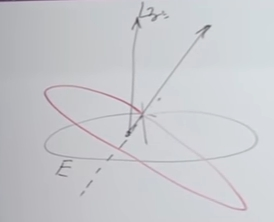
\includegraphics[width=0.5\textwidth]{aqm-2-1}
	\end{center}
\end{figure}

Let's look at the angular momentum generators. Figure \ref{fig:aqm-2-2} shows a  rotation about the z-axis by a small angle $\epsilon$.

\begin{figure}[H]
	\begin{center}
		\caption{Rotation in 2D by a small angle $\epsilon$}\label{fig:aqm-2-2}
		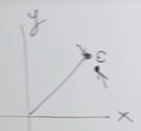
\includegraphics[width=0.5\textwidth]{aqm-2-2}
	\end{center}
\end{figure}

\begin{align*}
	\delta x =& - y \epsilon\\
	\delta y =& x \epsilon \text{. Now for a wave function $\psi(x,y)$}\\
	\delta \psi =& \frac{\partial \psi}{\partial x} \delta x + \frac{\partial \psi}{\partial y} \delta y\\
	=&\big( - y \frac{\partial \psi}{\partial x} + x \frac{\partial \psi}{\partial y}\big) \epsilon\\
	\triangleq& i \epsilon L_z \psi\\
	=& \big(- y P_x + x P_y x\big) i \epsilon \text{, whence}\\
	L_z =& x P_y - y P_x \text{, similarly}\\
	L_x =& y P_z - z P_y \text{, and}\\
	L_y =& x P_x - x P_z \text{, c.f. the classical formula}\\
	\vec{L} =& \vec{r} \times \vec{P}
\end{align*}
These are symmetries if the system is rotationally invariant.

Do they commute with each other? In \cite{susskind2014quantum} we saw
\begin{align*}
	[L,H_i]=& 0 \numberthis \label{eq:LH}\\
	[L_x,L_y] =& i L_z \numberthis \label{eq:lx_ly}\\
	[L_y,L_z] =& i L_x\numberthis \label{eq:ly_lz}\\
	[L_z,L_x] =& i L_y\numberthis \label{eq:lz_lx}
\end{align*}

\begin{defn}[Algebra]
	In mathematics, an \emph{algebra over a field } (often simply called an algebra) is a vector space equipped with a bilinear product. 
\end{defn}

\begin{defn}[Lie algebra]
	A Lie algebra is an algebra where multiplication is commutation. LS uses the definition that is is a collection of generators that is closed under commutation.
\end{defn}

So $L_x$, $L_y$, $L_z$ generate a Lie algebra: if we continue commuting we don't find anything new.

We want to find eigenvalues of angular momentum. It us useful to introduce creation and annihilation operators for $L_z$.
\begin{align*}
	L_{\pm} \triangleq& L_x \pm i L_y \numberthis \label{eq:comm:Lpm}\\
	[L_{\pm},L_Z] =& \mp L_{\pm} \numberthis \label{eq:comm:LpmLz}
\end{align*}

\begin{thm}[If $\ket{m}$ is an eigenvector of $L_z$, so are $L_+ \ket{m}$ and $L_- \ket{m}$]
	If 
	\begin{align*}
		L_z \ket{m} =& m \ket{m} \text{, then }\\
		L_z (L^+ \ket{m}) =& (m+1) (L^+\ket{m}) \text{, and}\\
		L_z (L^- \ket{m}) =& (m-1) (L^-\ket{m})
	\end{align*}
\end{thm}
\begin{proof}
	Suppose we have found one eigenvector of $L_z$:
	\begin{align*}
		L_z \ket{m} =& m \ket{m} \text{, magnetic quantum number}\numberthis \label{eq:ev:Lz}\\
		[L_+,L_z] \ket{m} =& \big(L_+L_z - L_zL_+\big) \ket{m}\\
		=&- L_+ \ket{m} \text{, from (\ref{eq:comm:LpmLz}). Rearranging  and using (\ref{eq:ev:Lz})}\\
		m L_+\ket{m} + L_+\ket{m} =& L_z L_+ \ket{m} \text{, whence}\\
		\big(m + 1 \big)L_+\ket{m}  =& L_z L_+ \ket{m} \text{; $L_+ \ket{m}$ is an eigenvector, eigenvalue $m+1$}\numberthis \label{eq:create_m}
	\end{align*}
	Similarly, $L_- \ket{m}$ is an eigenvector, eigenvalue $m-1$. The sequence of eigenvectors terminates if  $L_{\pm} \ket{m}=0$.
\end{proof}

So, using the algebra of commutators, we have generated a spectrum of values of $L_z$, separated by integers--see Figure \ref{fig:aqm-2-3}. Imagine that we rotate by $180\degree$: this takes $L_z\rightarrow - L_z$, so rotational symmetry requires that the termination points be reversed: they must be symmetrical. There are two possibilities--Figures \ref{fig:aqm-2-3a} and \ref{fig:aqm-2-3b}. We can show that the only values that are allowed for orbital angular momentum are integral (single values wave function), but half integral is also possible for spin. 

\begin{figure}[H]
	\caption{Spectrum of $L_z$.}\label{fig:spectrum_Lz}
	\begin{subfigure}[t]{0.3\textwidth}
		\caption{Terminators in red}\label{fig:aqm-2-3}
		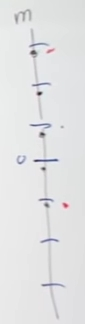
\includegraphics[width=0.8\textwidth]{aqm-2-3}
	\end{subfigure}
	\begin{subfigure}[t]{0.3\textwidth}
		\caption{Integral values in red}\label{fig:aqm-2-3a}
		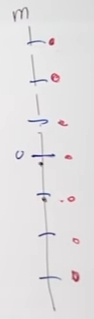
\includegraphics[width=0.8\textwidth]{aqm-2-3a}
	\end{subfigure}
	\begin{subfigure}[t]{0.3\textwidth}
		\caption{Half integral values}\label{fig:aqm-2-3b}
		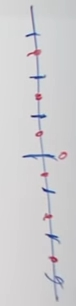
\includegraphics[width=0.8\textwidth]{aqm-2-3b}
	\end{subfigure}
\end{figure}

 We now show that the multiplet of states in Figure \ref{fig:aqm-2-3a} all have the same energy. 

\begin{thm}[Eigenvectors of $L_z$ are degenerate eigenvectors of $H$]
	\begin{align*}
	L_z \ket{m} = m \ket{m} \land& H \ket{m} = E \ket{m}\\
	 \implies&\\
	  H \ket{m \pm 1} =& E \ket{m \pm 1}
	\end{align*}
\end{thm} 
\begin{proof}
	\begin{align*}
	H \ket{m} =& E \ket{m} \numberthis \label{eq:assume_ev}\\
	H L_+ \ket{m} =& L_+ H \ket{m}\\
	=& L_+ E \ket{m} \text{, from (\ref{eq:assume_ev})}\\
	=& E L_+  \ket{m}\\
	H \ket{m+1} =& E \ket{m+1} \text{, from (\ref{eq:create_m})}
	\end{align*}
	Since symmetries commute, we have degeneracy.
\end{proof}

\section{Atomic orbits and harmonic oscillators}

\subsection{Atomic orbits and Angular Momentum}

We will talk more about what angular momentum is about.

If a particle moves in a central force field, angular momentum and, hence, the orbital plane are preserved. The state is $\psi(r,\theta,\phi)= \psi(r,\theta)$; if system were 2 dimensional, the angular momentum would be:

\begin{align*}
	L =& -i \frac{\partial}{\partial \theta} \text{, and the eigenvalues and eigenvectors would satisfy}\\
	-i \frac{\partial \psi(r,\theta)}{\partial \theta} =& l \psi(r,\theta) \text{, which has solution}\\
	\psi(r,\theta) =& e^{i l \theta} \chi(r) \text{, for some $\chi$}
\end{align*}

In 3 dimensions, $\psi(r,\theta,\phi)= Y(\theta,\phi) \chi(r)$, where $Y(\theta,\phi)$ encapsulates the angular dependence of the wave function.

In Section \ref{seq:symmetry:degeneracy} we derived the commutators, (\ref{eq:lx_ly}), (\ref{eq:ly_lz}), and (\ref{eq:lz_lx}). We selected one component, $L_z$, and worked with its eigenvectors, $L_z \ket{m} = m \ket{m}$. We defined $L_\pm$, (\ref{eq:comm:Lpm}), and found that they had useful properties, (\ref{eq:comm:LpmLz}). $L_\pm$ were raising and lowering operators, which take use up and down the spectrum.

We asked whether the raising and lowering could go on forever. The only way to come to an end is if $\exists l$ such that $L_+\ket{k}=0$ (and similarly for $L_-$). Spectrum has to be symmetric (rotational invariance). We found spectrum had to go up in integers, and that it started at either an integer or half integer. We found that the spectrum was a multiplet of $2l+1$ states. The multiplet is characterized by the magnitude of angular momentum.


From (\ref{eq:create_m}) we have a spectrum of angular momenta, integral or half integral, say $\set{-l,...,l:L_+\ket{l}=0}$. There are $2l+1$ states with constant $L^2 = L_x^2 + L_y^2 + L_x^2$. Classically $L^2 = L_z^2 +(L_x-iL_y)(L_x+iL_y)$, but this fails in quantum mechanics as they operators don't commute.

The quantum version is:
\begin{align*}
	L^2 =& L_z^2 +(L_x-iL_y)(L_x+iL_y) -i [L_x,L_y]\\
	=& L_z^2 + L_z + L^-L^+\\
	L^2\ket{l}=& L_z^2\ket{l} + L_z\ket{l} + L^-L^+\ket{l}\\
	=& l^2\ket{l} + l\ket{l} + 0\text{, because eigenvectors.}\\
	L^2\ket{l}=&l (l+1) \ket{l} \numberthis \label{eq:max:L}
\end{align*}

\begin{thm}[Degeneracy of $L^2$]\label{thm:degeneracy:L2}
	\begin{enumerate}
		\item $[L^2, L_i] =0$\label{thm:degeneracy:1}
		\item All eigenvectors of $L_z$ are eigenvectors of $L^2$, eigenvalue $l(l+1)$\label{thm:degeneracy:2}
	\end{enumerate}
\end{thm}
\begin{proof}
	Part \ref{thm:degeneracy:1}
	\begin{align*}
		[L^2, L_x] =& [L_x^2+L_y^2+L_2^2,L_x]\\
		=& \cancel{[L_x^2,L_x]} + [L_y^2,L_x] + [L_z^2,L_x] \numberthis \label{eq:L2}\\
		[L_y^2,L_x]=&L_yL_yL_x -L_y L_x L_y + L_y L_x L_y -L_xL_yL_y\\
		=&-L_y[L_x,L_y]-[L_x,L_y]L_y\\
		=&-iL_yL_z-iL_zL_y \text{, using (\ref{eq:lx_ly})} \numberthis \label{eq:ly2x}\\
		[L_z^2,L_x]=&L_zL_zL_x -L_z L_x L_z + L_z L_x L_z -L_xL_zL_z\\
		=&L_z[L_z,L_x]+[L_z,L_x]L_z\\
		=&iL_zL_y+iL_yL_z \text{, using (\ref{eq:lz_lx})} \numberthis \label{eq:lz2x}\\
		[L^2, L_x] =&0 \text{, on substituing (\ref{eq:ly2x}) and (\ref{eq:lz2x}) in (\ref{eq:L2})}
	\end{align*}
	Part \ref{thm:degeneracy:2}. We know from (\ref{eq:max:L}) that the eigenvector of $L_z$ with the maximum eigenvalue satisfies the  theorem. The theorem follows by induction once we have the following Lemma.
	\begin{lemma}[Induction step for Theorem \ref{thm:degeneracy:L2}]
		If $\ket{m}$ is an eigenvector of $L_z$, and it is also an eigenvector of $L^2$, with eigenvalue $l(l+1)$, and $L_-\ket{m}$ is not zero, then  $L_-\ket{m}$ is an eigenvector of $L^2$, with eigenvalue $l(l+1)$.
	\end{lemma}
	\begin{proof}
		\begin{align*}
		L^2\ket{m}=&l (l+1) \ket{m} \text{, by hypothesis. Now}\\
		[L_-,L^2] =& 0 \text{, from (\ref{eq:comm:Lpm}) and Part \ref{thm:degeneracy:1}, hence}\\
		L^2(L_- \ket{m})=&(L^2 L_-) \ket{m}\\
		=& (L_- L^2) \ket{m}\\
		=& L_- (L^2 \ket{m})\\
		=& L_- [l (l+1) \ket{m}]\\
		=& l (l+1) (L_- \ket{m})
		\end{align*}
	\end{proof}
	
\end{proof}

When we find a multiplet such as Figure \ref{fig:aqm-2-3}, we not only have eigenvectors of $L_z$, but also of $L^2$. For each $l $, there are $2l+1$ states with the same $L^2$, and the same Energy\footnote{Because $[L_i,H]=0$--(\ref{eq:LH})}. Classically they are just tilts--Figure \ref{eq:aqm-2-1}.

We have a collection of functions of the angles, characterized by $m$ and $l$, $Y_{ml}(\theta,\phi)$. They are known as ''spherical harmonics'', and they are the analogues on the unit sphere of $e^{\pm i l \theta}$

\subsection{The Central Force Problem}

We will use classical mechanics to guess a solution.


Classically:
\begin{align*}
	H =& \frac{\vec{P}^2}{2m} + V(r) \text{, conserved} \numberthis \label{eq:classical:Hamiltonian}\\
	\vec{L} =& \vec{r}\times \vec{P}  \text{, angular momentum is conserved, so use $xy$ plane}\\
	H =& \frac{P_r^2+P_{\theta}^2}{2m} +V(r) \text{, resolving as shown in Figure \ref{fig:aqm-3-1-momentum}} \numberthis \label{eq:resolve}\\
	=& \frac{P_r^2}{2m} + \frac{L^2}{2m r^2} + V(r) \text{, since $\left|L\right| = \left|r\right| \left|P\right|$}
\end{align*}

So we have an equation for a one dimensional problem. Figure \ref{fig:aqm-3-central} depicts the potential, and Figure \ref{fig:aqm-3-central-osc} shows a solution, oscillations about the $r$ that yields the minimum potential. 

\begin{figure}[H]
	\caption{Central Force as  a one dimensional problem}
	\begin{subfigure}[t]{0.3\textwidth}
		\caption{Resolving momentum into radial and angular components}\label{fig:aqm-3-1-momentum}
		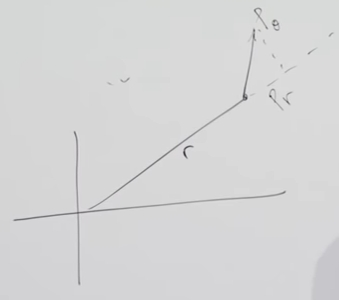
\includegraphics[width=\textwidth]{aqm-3-1-momentum}
	\end{subfigure}
	\begin{subfigure}[t]{0.3\textwidth}
		\caption{Potential assuming the Coulomb force}\label{fig:aqm-3-central}
		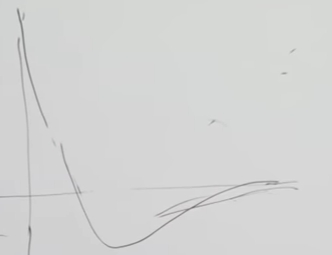
\includegraphics[width=\textwidth]{aqm-3-central}
	\end{subfigure}
	\begin{subfigure}[t]{0.3\textwidth}
		\caption{Small oscillations about minimum}\label{fig:aqm-3-central-osc}
		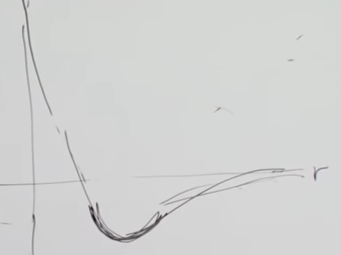
\includegraphics[width=\textwidth]{aqm-3-central-osc}
	\end{subfigure}
\end{figure}

That is the classical physics. What about the quantum physics? For the quantum physics we have a wave function which satisfies the Schr\"odinger Equation(\ref{eq:schroedinger:central}). The angular part is totally taken care of by our existing study of angular momentum\footnote{Strictly step (\ref{eq:resolve}) requires a quantum mechanical justification}.
\begin{align*}
	-\frac{\hslash^2}{2m}\frac{\partial^2 \psi(r)}{\partial r^2} + \hslash^2 \frac{l(l+1)\hslash^2}{r^2}\psi(r)+V(r)\psi(r) =& E\psi(r)\numberthis \label{eq:schroedinger:central}
\end{align*}

Figure \ref{fig:aqm-3-central-potential} depicts the potential for the Coulomb force. The energy levels of (\ref{eq:schroedinger:central}) are characterized by the number of nodes--Definition \ref{defn:node} and Figures \ref{fig:aqm-3-central-0node}, \ref{fig:aqm-3-central-1node}, and \ref{fig:aqm-3-central-2nodes} (The more nodes, the faster the wiggle, hence higher momentum).

\begin{figure}[H]
	\caption{Solving Central Potential Schro\"dinger Equation (\ref{eq:schroedinger:central})}
	\begin{subfigure}[t]{0.45\textwidth}
		\caption{Potential}\label{fig:aqm-3-central-potential}
		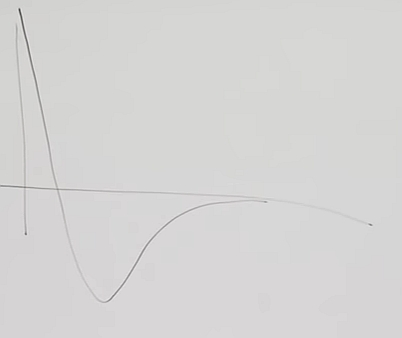
\includegraphics[width=\textwidth]{aqm-3-central-potential}
	\end{subfigure}
	\begin{subfigure}[t]{0.45\textwidth}
		\caption{No nodes}\label{fig:aqm-3-central-0node}
		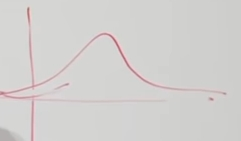
\includegraphics[width=\textwidth]{aqm-3-central-0node}
	\end{subfigure}
	\begin{subfigure}[t]{0.45\textwidth}
		\caption{One node}\label{fig:aqm-3-central-1node}
		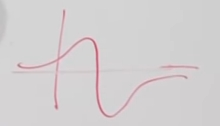
\includegraphics[width=\textwidth]{aqm-3-central-1node}
	\end{subfigure}
	\begin{subfigure}[t]{0.45\textwidth}
		\caption{Two nodes}\label{fig:aqm-3-central-2nodes}
		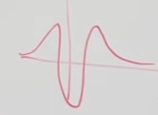
\includegraphics[width=\textwidth]{aqm-3-central-2node2}
	\end{subfigure}
\end{figure}

\begin{defn}[Node]\label{defn:node}
	A node is a point where the wave function is zero.
\end{defn}

\begin{thm}[Nodes and energy levels]
	The ground state has 0 nodes, the first excited one node, etc.
\end{thm}

What can we say about energy levels in general? Figure \ref{fig:degeneracy:hydrogen} plots the number of energy levels against $l$, and plots number of nodes vertically. It exhibits degeneracy. If the energy is too high the electron escapes. The Coulomb potential has a very special feature. It is almost an accident: it is violated by the finite size of the nucleus, by relativistic corrections, by spin. \emph{The zero node energy for $l=1$ is equal to the 1 node energy for $l=0$, etc}--Figure \ref{fig:aqm-3-central-coulomb}.



\begin{figure}[H]
	\begin{center}
		\caption[Degeneracy of Energy Levels in Hydrogen Atom]{Degeneracy of Energy Levels in Hydrogen Atom. Each $l$ has its own Schro\"edinger equation (\ref{eq:schroedinger:central}), so each $l$ may have its own set of bound solutions. The ground state for $l=0$ has no nodes,  the next state has one node, etc. For $l=1$ the energy of the ground state lies somewhere above the corresponding state for $l=1$. Moreover there are 3 states for each node: the energy levels are degenerate. Similarly for $l=2$ there are 5 states for each node, and the energy levels are higher.}\label{fig:degeneracy:hydrogen}
		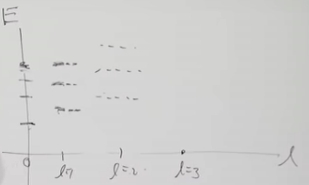
\includegraphics[width=0.9\textwidth]{aqm-3-hydrogen-degeneracy}
	\end{center}
\end{figure}

\begin{figure}[H]
	\begin{center}
		\caption[Energy Levels for the Coulomb Force]{For the Coulomb force \emph{only}, the energy levels for $l+1$ match those for $l$, shifted up by one. This is an extra degeneracy from a bizarre symmetry. The number of states at each level is  $\{1,4,9,16,...\}$}\label{fig:aqm-3-central-coulomb}
		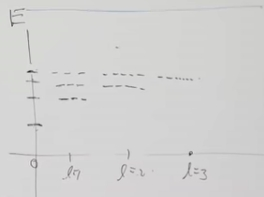
\includegraphics[width=0.8\textwidth]{aqm-3-central-coulomb}
	\end{center}
\end{figure}

Real atoms behave a bit differently.
\begin{itemize}
	\item the nucleus has finite size, so at short distances the Coulomb law isn't quite accurate;
	\item Instead of  $\{1,4,9,16,...\}$ states at each energy level there are  $\{2,8,18,32,...\}$--we have ignored \emph{spin}.
\end{itemize}

Are there always raising an lowering operators? No: only when you are very lucky; physics has been lucky twice. The harmonic oscillator piece of luck is very pervasive, as many things in nature can be well approximated by a harmonic oscillator. For example, go to a higher momentum state of the central force problem, Figure \ref{fig:aqm-3-central-osc}, and the simplest solution is to treat them as a harmonic oscillator.

\subsection{Harmonic oscillators}\label{sect:harmonic:oscillators}


Everything in physics that has an equilibrium, if you disturb equilibrium by a small amount, the behaviour can be approximated by a  harmonic oscillator. The model is just a suspended mass $(m=1)$, spring constant $(k=\omega^2)$

\begin{figure}[H]
	\begin{center}
		\caption[Model: suspended mass.]{Suspended mass $(m=1)$, spring constant $(k=\omega^2)$.  $X$ is deviation from equillibrium.}\label{fig:aqm-3-shm-suspended-mass}
		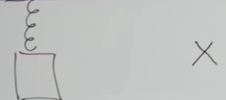
\includegraphics[width=0.8\textwidth]{aqm-3-shm-suspended-mass}
	\end{center}
\end{figure}

Classically:
\begin{align*}
	H =& \frac{P^2}{2m} + \frac{\omega^2 x^2}{2} \text{. We'll check with Hamilton's equations}\\
	 \dot{p}=&\frac{\partial H}{\partial x} \\
	=& \dot{x} \\
	\dot{x} =& -\frac{\partial H}{\partial p} \\
	=& - \omega^2 p \\
	\dddot{x} + \omega^2 x =&0 \text{, as expected}
\end{align*}

Quantum mechanically:
\begin{align*}
	H =& \frac{P^2}{2m} + \frac{\omega^2 x^2}{2}\\
	=& \frac{\omega}{2 \omega}\big(P + i \omega x \big)\big(P - i \omega x \big) - \frac{i \omega}{2} [x,P] \text{, since x and p don't commute}\\
	=& \frac{\omega}{2 \omega}\big(P + i \omega x \big)\big(P - i \omega x \big) + \underbrace{\frac{\hslash \omega}{2}}_\text{zero point energy}\\
	=&\omega \frac{\big(P + i \omega x \big)}{\sqrt{2 \omega}}\frac{\big(P - i \omega x \big)}{\sqrt{2 \omega}}
\end{align*}

Classically both $p=0$ and $x=0$ in the ground state; since the Heisenberg uncertainty principle precludes  $p=0$ and $x=0$, the zero point energy is the minimum possible. We'll drop the ground state energy (zero point energy) for the time being, since it is just an additive constant\footnote{At the end of lecture \ref{section:fermions:dirac}, LS mentioned that the zero point energy is involved only in gravitational interactions; elsewhere only the energy \emph{difference} matters}.

We'll introduce raising and lowering operators:

\begin{align*}
	a^+ \triangleq & \frac{P + i \omega x } {\sqrt{2 \omega}} \numberthis \label{eq:creation:operator}\\
	a^- \triangleq & \frac{P - i \omega x } {\sqrt{2 \omega}}\text{, Hermitean conjugate--$a^-=(a^+)^\dagger$} \numberthis \label{eq:annihilation:operator}\\
	H =& \omega a^+ a^-\text{. We'll take the commutator:}\numberthis \label{eq:shM}\\
	[a^-,a^+] =& \frac{1}{2\omega}\big[P - i \omega x,P + i \omega x\big]\\
	=& 1\text{. We also define} \numberthis \label{eq:a:comm}\\
	N \triangleq& a^+a^-\text{, so (\ref{eq:shM}) becomes} \numberthis \label{eq:number:operator}\\
	H =& \omega N
\end{align*}
$N$ is Hermitian, so it has a complete set of eigenvalues and eigenvectors.

\begin{align*}
	N\ket{n} =& n\ket{n} \text{, we aren't \emph{assuming} that $n$ is an integer}\\
	a^+a^-\ket{n} =& n\ket{n}\\
	a^+(a^-a^+ - a^+a^-)\ket{n} =& a^+\ket{n}\text{, using (\ref{eq:a:comm})}\\
	a^+a^-a^+ \ket{n} - a^+\underbrace{a^+a^- \ket{n}}_\text{$ n\ket{n}$} =& a^+\ket{n}\\
	\underbrace{a^+a^-}_\text{$N$}a^+ \ket{n} =& n a^+\ket{n} + a^+\ket{n}\\
	N a^+ \ket{n} =& (n+1) a^+ \ket{n}
\end{align*}

So $a^+$ acts as raising operator, and we can show $a^-$ is lowering.  Since the Hamiltonian is positive we can't ever get negative energy, so there must be a lowest energy state, $0$--Figure \ref{fig:aqm-3-spectrum}. In QM there is a theorem that all the eigenvalues of $MM^\dagger$ are positive or zero, for any operator $M$. 

\begin{figure}[H]
	\begin{center}
		\caption[Energy Spectrum for Harmonic Oscillator]{Energy Spectrum for Harmonic Oscillator. $a^+$ takes energy up one level, and $a^-$ down, except for $a^-\ket{0}$=0.}\label{fig:aqm-3-spectrum}
		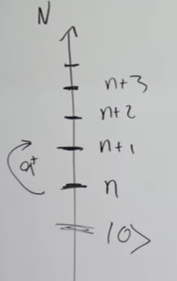
\includegraphics[width=0.8\textwidth]{aqm-3-spectrum}
	\end{center}
\end{figure}
We will see (Theorem \ref{thm:norm:harmonic}) the appropriate normalization gives:
\begin{align*}
	a^+\ket{n} =& \sqrt{n+1}\ket{n+1}\\
	a^-\ket{n} =& \sqrt{n}\ket{n-1}
\end{align*}
 
\section{Spin}

\subsection{Harmonic oscillators(continued)}

Harmonic oscillators are ubiquitous. Any time a system has an equilibrium, there can be oscillations about equilibrium. An oscillator can oscillate at different frequencies simultaneously (harmonics)--e.g. a violin string. We will be particularly interested in oscillations in an electromagnetic field.  For example, if you have radiation in a cavity, there will be a variety of oscillations. What is the equilibrium? No electromagnetic field, i.e. vacuum is the equilibrium for electromagnetic field. Give it a knock, e.g. microwaves, and there will be oscillations.

In a crystal, the oscillations of one atom affect its neighbours, so we have a field. The quanta are called phonons.

In Section \ref{sect:harmonic:oscillators} we found:
\begin{align*}
	H =& \frac{P^2}{2m} + \frac{\omega^2 x^2}{2} \text{, and we defined}\\
	a^\pm=& \frac{q \pm i \omega x}{\sqrt{2 \omega}} \text{, raising and lowering operators}\\
	[a^-,a^+]=& 1\\
	N =& a^+a^- \text{, whence}\\
	H =& \omega(N+\frac{1}{2})
\end{align*}

We will find ground state by solving the Schr\"odinger equation.
\begin{align*}
	\ket{\psi} \rightarrow& \psi_0(x) \text{, in thr ground state}\\
	X \rightarrow& x. \text{, multiplication}\\
	P \rightarrow& -i \frac{d}{dx}
\end{align*}


We know that there has to be a ground state. We can't use $a^-$ indefinitely; since $H$ is positive, there can be no negative eigenvalues. So $\exists \ket{0}$ such that: 
\begin{align*}
	a^-\ket{0}=&0\\
	N\ket{0}=&a^+a^- \ket{0 }\\
	=& a^+0\\
	=&0
\end{align*}

NB $\ket{0} \ne 0$. $\ket{0}$ is a vector which can be normalized; $0$ is a vector of length 0.
Applying the transformations given above, we get the time independent Schr\"odinger equation.
\begin{align*}
	-\frac{1}{2}\frac{d^2 \psi(x)}{dx^2} + \omega^2 x^2 \psi(x)=& E\psi(x)
\end{align*}

 There are solutions for all $E$, but the solutions are not normalizable unless E is in the spectrum, Figure \ref{fig:aqm-3-spectrum}. So we impose the condition $\braket{\psi|\psi}=1$, or:
\begin{align*}
	\int_{-\infty}^{\infty} dx \psi^*(x) \psi(x) =& 1 \text{. We know that}\\
	a^-\ket{0}=& 0 \text{, whence}\\
	\big(-i \frac{d}{dx} - i \omega x \big)\psi_0(x) =& 0 \text{. Write}\\
	\psi(x)=&e^{f(x)} \text{, then}\\
	\psi^\prime(x) =&f^\prime e^{f(x)}\\
	i \big[f^\prime  + \omega x\big]e^{f(x)} =&0\\
	f(x) =& -\frac{\omega x^2}{2}+C\\
	\psi_0(x) =& e^{-\frac{\omega x^2}{2}} \text{, not normalized.}
\end{align*}

We can then use $a^+$  to generate excited states.
\begin{align*}
	\ket{1}=& a^+ \ket{0} \text{, or, in the Schro\"edinger representation:}\\
	\psi_1(x) =& \big(-i \frac{d}{dx} + i \omega x \big) e^{-\frac{\omega x^2}{2}}\\
	=& 2 i \omega e^{-\frac{\omega x^2}{2}}
\end{align*}

This is an odd function (antisymmetric)--Figure \ref{fig:wave:harmonic}. It has one node.

Figure \ref{fig:wave:harmonic} shows how higher levels have more wiggles (momentum) and are away from origin (the particle is more likely to be far away) most of time.

\begin{figure}[H]
	\caption{Wave functions for harmonic oscillator}\label{fig:wave:harmonic}
	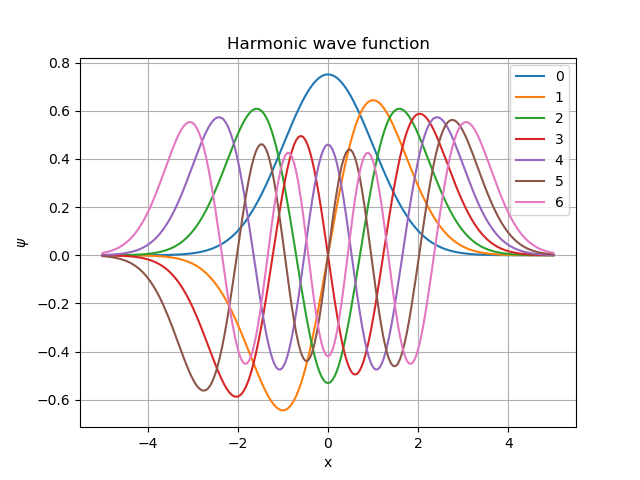
\includegraphics[width=0.9\textwidth]{harmonic_wavefunction}
\end{figure}

To see classical behaviour, superpose states to create wave packets. Time dependent looks like classical oscillator, especially at high energy (energy larger that ground state).



\subsection{Spin}

Some particles have half-integral spin, e.g. electron or proton. At rest they have no orbital rotation, no $\vec{r}\times\vec{p}$, only spin. Spin is a kind of angular momentum that is attached to a particle. You can think of it as an abstract quantity or as a tiny thing that is literally spinning. It transforms under rotation as angular momentum does. Spin has two states, up or down, left or right, in or out. The thing that characterizes angular momentum is having three components, which can be represented by matrices satisfying (\ref{eq:lx_ly}), (\ref{eq:ly_lz}), and (\ref{eq:lz_lx}). These are closely related to the commutation relations of the Pauli matrices (we will work in the representation of the $z$ component of the spin):

\begin{align*}
	\sigma_z =& \begin{pmatrix}
		1 & 0 \\
		0 & -1\\
	\end{pmatrix} \\
	\sigma_x =& \begin{pmatrix}
		0 & 1 \\
		1 & 0\\
	\end{pmatrix}\\
	\sigma_y =& \begin{pmatrix}
		0 & -i \\
		i & 0\\
	\end{pmatrix}
\end{align*}

The Pauli matrices are Hermitian. We define:

\begin{align*}
	\vec{s} =& \frac{\vec{\sigma}}{2} 
\end{align*}

We can show the $s_i$ satisfy (\ref{eq:lx_ly}), (\ref{eq:ly_lz}), and (\ref{eq:lz_lx}).

\begin{align*}
	[s_x,s_y] =& i s_z \\
	[s_y,s_z] =& i s_x\\
	[s_z,s_x] =& i s_y
\end{align*}
So the Pauli matrices, operating on 2D vectors, represent a simple angular momentum system, which is attached to the particles. Now we can ask about eigenvalues and eigenvectors. The Eigenvalues of $s_z$ are $\pm \frac{1}{2}$. 

In Figures \ref{fig:aqm-2-3a} and \ref{fig:aqm-2-3b} we saw there were two possibilities for the spectrum of angular momentum, integral and half integral spins. We could have \emph{guessed} the Pauli matrices by noticing the spin ${-\frac{1}{2},\frac{1}{2}}$ case. Note: there are spin $0$ particles, such as the Higgs, and the deuteron. We will largely focus on spin $\frac{1}{2}$ particles.

We define $J$, the total angular momentum:
\begin{align*}
	J=&L+s \text{, where $L$ denotes the orbital angular momentum $\vec{r}\times\vec{P}$}
\end{align*}

There are QM rules for adding angular momenta, which we won't cover in this lecture.


The first experimental background came from spectroscopy and the periodic table. The goal of this lecture is to see how periodic table emerges from spin. Pauli realized spin was needed.

$L^2=l(l+1)$. We look at the energy levels of hydrogen --see Figure \ref{fig:degeneracy:hydrogen}. There is a bunch of states for $l=0$, for zero nodes($n=0$), 1 node, etc. For $l=1$ there are $2l+1=3$ states for each node, and ground state for $l=1$ has more energy than ground state for $l=0$, because it has angular momentum.

Figure \ref{fig:aqm-3-central-coulomb} shows the coincidence that the  energy for  for one value of $l$ matches that $l-1$, except that energies are shifted in $n$: $E(n,l)$ satisfies $E(n,l+1)=E(n+1,l)$. So the number of states for each n is 1, 4, 9, 16, ...

The Helium nucleus has twice the charge of the hydrogen nucleus, so electrons are pulled in tighter, but the structure of Figure \ref{fig:aqm-3-central-coulomb}  is preserved for a Helium ion (negative). Put another electron in: we can put 2 electrons into ground state; if we try to create an ion with 3 electrons, one goes into first excited state! 

\subsection{Pauli exclusion principle}

Pauli exclusion principle: no two electrons can ever get into the same state. But we can put 2 electrons into ground state. Pauli said there was a new property with two values, up and down.

Lithium has 3 electrons, 2 in ground state, 3rd in 1st excited state. There is room for 8 states in first excited level, if we allow for spin. This explains 2nd row of periodic table. The fact that spin was angular momentum was checked with magnetic field (split energy levels).

Pauli's Exclusion Principle is a \emph{postulate} of non-relativistic QM, but a \emph{consequence} of relativistic QM. There are two kinds of particles: ones that satisfy Pauli's Exclusion Principle (Fermions), and those that don't (Bosons).

In statistical mechanics, how do we handle identical particles? Imagine that we are putting particles into boxes (real or phase space). In Figure \ref{fig:aqm-4-particles-boxen} we can imagine each particle having a name painted in "classical paint", so they are distinct. Or we can treat them as absolutely identical, so we usually count as if they were identical. In quantum mechanics, however, identical  particles are indistinguishable.

\begin{figure}[H]
	\begin{center}
		\caption[Configurations Particles in Boxes]{Configurations Particles in Boxes: if we exchange labels, do we count as separate configurations?}\label{fig:aqm-4-particles-boxen}
		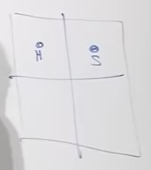
\includegraphics[width=0.6\textwidth]{aqm-4-particles-boxen}
	\end{center}
\end{figure}

Consider two particles, forgetting spin.
\begin{align*}
	\psi(x) =& \braket{x|\psi}\\
	\psi(x_1,x_2) =& \braket{x_1x_2|\psi}\text{, two particles}\\
	\psi(x_1,x_2) \rightarrow & \psi(x_2,x_1)\text{, swap using operator $S$}\\
	S\ket{x1,x2} =& \ket{x2,x1}\\
	S^2 =& 1
\end{align*}

$S$ is unitary, so eigenvalues are $\pm1$.

\section{Fermions: a tale of two minus signs}


We'll review the chemistry that went into the discovery of spin, and the Fermionic character of electrons. The Fermionic character implies two things that are related:
\begin{itemize}
	\item spin of electron is half spin $\pm \frac{1}{2}$
	\item the electron satisfies the Pauli Exclusion Principle.
\end{itemize} 

We can put 2 electrons into the ground state only because of spin. NB, the 2 electrons in Helium are \textit{entangled}.

Photons don't have an exclusion principle; in fact they have a tendency to congregate.
 
Can we have spin $\frac{1}{2}$ particles that don't obey Pauli exclusion principle, or a spin integer that does obey Pauli exclusion principle? No. Can show this from quantum field theory.

This lecture is a tale of two minus signs, one from exchange--Section \ref{section:swap},  the other from spin--Section \ref{section:spin}.

\subsection{Swapping particles}\label{section:swap}

The Pauli Exclusion Principle is deeper than simply saying that you cannot put two particles into the same state. It is actually a statement about multi particle wave functions. Let's forget about spin for the moment.

Consider wave function of positions for multiple particles, e.g. $\ket{x_1,x_2,x_3}$. Then $\braket{x_1,...x_n|\psi}=\psi(x_1,...x_n)$, and $\psi^*(x_1,...x_n)\psi(x_1,...x_n)$ is the probability that the system is in state $\ket{x_1,...x_n}$. We ask whether $\psi(x_1,x_2,...x_n)$ is the same as $\psi(x_2,x_1,...x_n)$, or, equivalently, whether the upper configuration in Figure \ref{fig:aqm-4-states} is the same as the lower one. All experiments and theory agree that they are the same state: $\ket{x1,x2}=\ket{x2,x1}$ .

\begin{figure}[H]
	\begin{center}
		\caption{Is the upper configuration the same as the lower one?}\label{fig:aqm-4-states}
		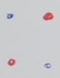
\includegraphics[width=0.8\textwidth]{aqm-4-states}
	\end{center}
\end{figure}

On the other hand, the physical properties of a state do not depend on the overall phase. We can't say that $\ket{x_1, x_2}=\ket{x_2, x_1}$, as there may be a phase $e^{i\phi}$.
\begin{align*}
	\ket{x_1, x_2}=&\ket{x_2, x_1}e^{i\phi}\text{, interchange twice--there are two possibilities}\\
	\ket{x_1, x_2}=&+\ket{x_2, x_1}\text{ Bosons}\\
	\ket{x_1, x_2}=&-\ket{x_2, x_1}\text{ Fermions}
\end{align*}

NB: sign is not observable.

\begin{table}[H]
	\begin{center}
		\caption{Wave functions for Fermions and Bosons}
			\begin{tabular}{|l| c| c|} \hline 
				Wave function&Fermions&Bosons \\ \hline 
				$\psi(x_1,x_2)=-\psi(x_2,x_1)$&OK&not OK\\ \hline
				$\psi(x_1,x_2)=\psi(x_2,x_1)$&not OK& OK\\ \hline
				$\psi_0(x_1)\psi_0(x_2)$&not OK& OK\\ \hline
				$\psi_0(x_1)\psi_1(x_2)$&not OK& not OK\\ \hline
				$\psi_0(x_1)\psi_1(x_2)+\psi_0(x_2)\psi_1(x_1)$&not OK& OK\\ \hline
				$\psi_0(x_1)\psi_1(x_2)-\psi_0(x_2)\psi_1(x_1)$&OK&not OK \\ \hline
		\end{tabular}
	\end{center}
\end{table}

When there is spin we can think of the wave function as a function of position and spin--$\psi(x,\sigma_z)$ and $\psi(x1,\sigma_1,x2,\sigma_2,...)$. You cannot put two Fermions into the same state.

\subsection{Spin}\label{section:spin}

Rotation by $2\pi$ is a mathematical process that you might expect to do nothing. Let's consider a wave function for one particle $\psi(x,\sigma)$ and rotate the coordinate system or the particle. What happens when you rotate a system with a given angular momentum by an angle about any axis--$R(\theta)2\pi$? What about $R(2\pi)2\pi$? Surely this leaves the system unchanged? But the system is analogous to swapping particles--Section \ref{section:swap}. If all we want is for the probabilities and expectation to be preserved, perhaps the rotations introduce a phase--$\pm1$.

Consider the generator of rotations:
\begin{align*}
	J_z\ket{\psi} =& -i \frac{\partial \ket{\psi}}{\partial \theta}
\end{align*}
Imagine that angular momentum about $z$ has a definite value, so $\ket{\psi}$ is an eigenvector.
\begin{align*}
	J_z\ket{\psi}=& m\ket{\psi} \text{, which is easily solved.}\\
	\ket{\psi(\theta)} =& e^{im\theta}\ket{\psi(0)}
\end{align*}

But, from the commutation relations\footnote{See discussion preceding Figure \ref{fig:spectrum_Lz}} we know that  $m$ integral or half integral (in 3D, not 2D).
What if $m$ half integral and we rotate by $2\pi$? We have phase of $-1$, so $\psi$ changes sign. Fermions follow $-1$, Bosons $+1$. Of course rotation by  $4\pi$ does give the identity.

Leonard Susskind demonstrated that $2\pi\ne0$:
\begin{itemize}
	\item Gerard 't Hooft Coffee Cup--Figure \ref{fig:thooft:coffee_cup} 
	\item Dirac sphere in a box
\end{itemize}
In each case we are following a path in rotation space.

\begin{figure}[H]
	\caption{The Gerard 't Hooft Coffee Cup trick}\label{fig:thooft:coffee_cup}
	\begin{subfigure}{0.45\textwidth}
		\caption{Starting the first rotation}
		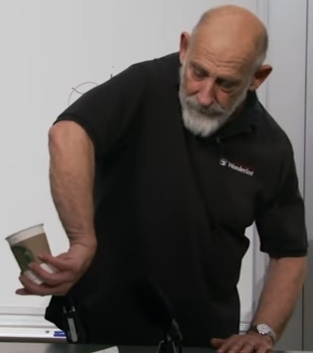
\includegraphics[width=\textwidth]{aqm-5-coffee-cup1}
	\end{subfigure}
	\begin{subfigure}{0.45\textwidth}
		\caption{$2\pi$: That is not the identity: let me tell you I'm quite certain that is not the identity!}
		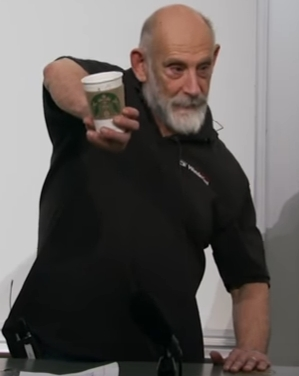
\includegraphics[width=\textwidth]{aqm-5-coffee-cup2}
	\end{subfigure}
	\begin{subfigure}{0.45\textwidth}
		\caption{Staring the 2nd rotation}
		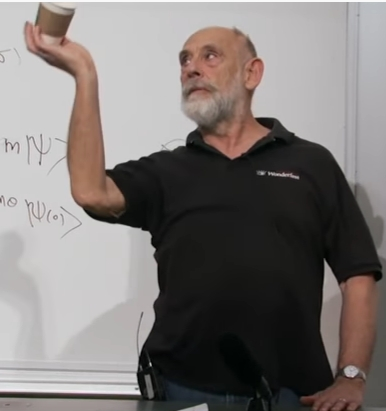
\includegraphics[width=\textwidth]{aqm-5-coffee-cup3}
	\end{subfigure}
	\begin{subfigure}{0.45\textwidth}
		\caption{$4\pi$: that is the identity}
		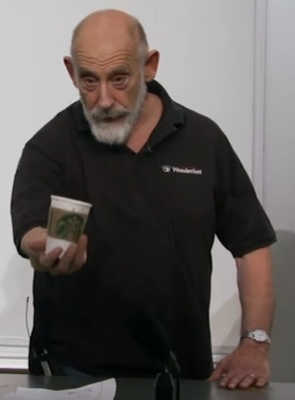
\includegraphics[width=\textwidth]{aqm-5-coffee-cup4}
	\end{subfigure}
\end{figure}

\begin{itemize}
	\item The wave function for two fermions changes sign when we swap them;
	\item The wave function for a single fermion changes sign when we rotate by $2\pi$.
\end{itemize}

\subsection{The connection between interchange and rotation}

Is there a connection between interchange and rotation? Yes: it was discovered by David Finkelstein. 

\begin{figure}[H]
	\caption[The David Finkelstein Belt Trick]{The David Finkelstein Belt Trick: A rotation by $2\pi$, plus an exchange, gives an untwisted belt}
	\begin{subfigure}[t]{0.5\textwidth}
		\caption{Exchange of the two loops}
		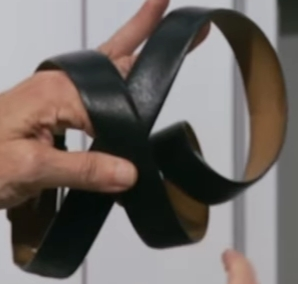
\includegraphics[width=\textwidth]{aqm-5-belt-exchange}
	\end{subfigure}
	\begin{subfigure}[t]{0.5\textwidth}
		\caption{Turn around and we see 2 rotations instead}
		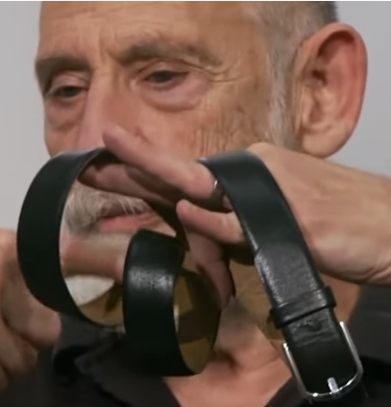
\includegraphics[width=\textwidth]{aqm-5-belt-rotation}
	\end{subfigure}
	\begin{subfigure}[t]{0.24\textwidth}
		\caption{Not a possible configuration from twisting a belt}
		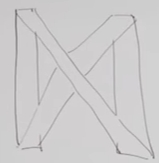
\includegraphics[width=\textwidth]{aqm-5-belt-illegal}
	\end{subfigure}
	\begin{subfigure}[t]{0.24\textwidth}
		\caption{The twist makes it legal: you can pull it apart to get the topologically trivial configuration.}
		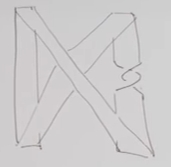
\includegraphics[width=\textwidth]{aqm-5-belt-legal}
	\end{subfigure}
	\begin{subfigure}[t]{0.24\textwidth}
		\caption{Add time, and create two pairs of particles at bottom}\label{fig:aqm-5-belt-legal-time}
		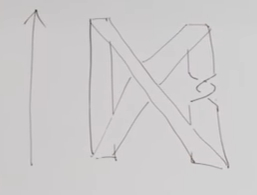
\includegraphics[width=\textwidth]{aqm-5-belt-legal-time}
	\end{subfigure}
	\begin{subfigure}[t]{0.24\textwidth}
		\caption{Rotate one particle, and switch two of them. The switch and rotate give the same configuration}\label{fig:belt_switch:rotate}
		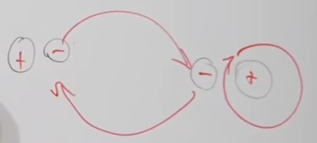
\includegraphics[width=\textwidth]{aqm-5-belt-switch-rotate}
	\end{subfigure}
\end{figure}


This shows the deep topological connection between rotation and interchange.

Imagine that I have two particles. I take one at rotate it by $2\pi$, then I switch two of them. Then, regardless of whether they are Fermions or Bosons, doing nothing is equivalent to doing a rotation and an exchange--Figure \ref{fig:belt_switch:rotate} (this isn't the way Pauli did it).

This would not make sense if particles were eternal. Quantum Field Theory allows particles to be created. We start with no particles, then create particle-antiparticle pairs--Figure \ref{fig:aqm-5-belt-legal-time}. Do whatever it takes to create particles out of nothing. As time goes on, at the same time we rotate one particle and exchange the two negative ones. Topologically this is equivalent to just creating the two particles and not doing anything.

The spin statistics theorem is more general than the version Pauli proved. It is also true for solitons. A soliton is (solitary wave) is a lump of field (Finkelstein, Rubinstein). Its true for lumps of stuff in condensed matter physics, for manifolds, for all kinds of things where Pauli's argument doesn't apply.


Assume field is mostly zero, but there are lumps. The spin statistics theorem says that there are two kinds of lumps: those whose wave function changes sign when rotated, and those where it doesn't change--Figure \ref{fig:lump:antilump}--Fermions and Bosons.

\begin{figure}[H]
	\caption{Annihilation of lumps and anti-lumps}\label{fig:lump:antilump}
	\begin{subfigure}{0.3\textwidth}
		\caption{Blue and black lumps}
		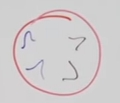
\includegraphics[width=\textwidth]{aqm-5-lumps}
	\end{subfigure}
	\begin{subfigure}{0.3\textwidth}
		\caption{Mirror image}
		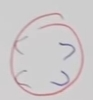
\includegraphics[width=\textwidth]{aqm-5-anti-lumps}
	\end{subfigure}
	\begin{subfigure}{0.3\textwidth}
		\caption{Bring together - black lumps annihilated}
		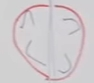
\includegraphics[width=\textwidth]{aqm-5-partially-annihilated}
	\end{subfigure}
\end{figure}

Is there a way to observe the change in phase of a Fermion?

Let's start with a experiment where you wouldn't see anything. Put electron in a cavity with a magnetic field, \emph{slowly} rotate box, release, and generate interference pattern--Figure \ref{fig:aqm-5-expt1}. Compare with another experiment where we don't rotate: the interference pattern won't show any differences--Figure \ref{fig:aqm-5-expt-beam-splitter}. Now use a beam splitter, and we see interference from the $2\pi$ rotation (we don't know which box contains electron: don't look!).

Repeat with a beam splitter
\begin{figure}[H]
	\caption {An experiment to observe the change in phase of a Fermion}
	\begin{subfigure}[t]{0.3\textwidth}
		\caption{Two experiments, with an without \emph{slow} rotation}\label{fig:aqm-5-expt1}
		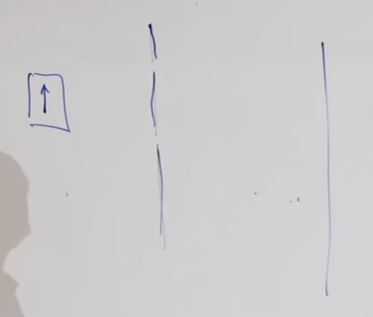
\includegraphics[width=\textwidth]{aqm-5-expt1}
	\end{subfigure}
	\begin{subfigure}[t]{0.3\textwidth}
		\caption{Experiment with beam splitter: one electron, but waves are split. One box \emph{only} rotates. $\psi_1(x)-\psi_2(x)\ne\psi_1(x)+\psi_2(x)$}\label{fig:aqm-5-expt-beam-splitter}
		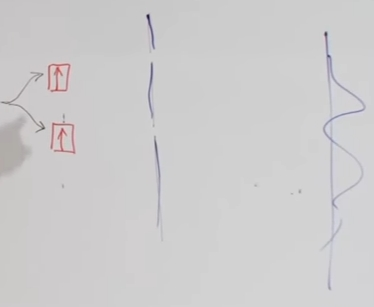
\includegraphics[width=\textwidth]{aqm-5-expt-beam-splitter}
	\end{subfigure}
	\begin{subfigure}[t]{0.3\textwidth}
		\caption{Detail of actual experiment. Magnetic field used to rotate spin, tuned so rotation is $2\pi$}
		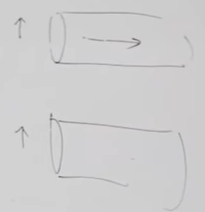
\includegraphics[width=\textwidth]{aqm-5-expt-actual}
	\end{subfigure}
\end{figure}



\section{Quantum Field Theory}

We are entering today into the world of Quantum Field Theory. Quantum Field Theory is the description of nature as we know it, with the exception of gravity. In principle we believe that we could explain everything, except gravity, if we only had enough computational power. Of course problems tend to be too complicated. We can understand hydrogen, but boron is already too complicated, and human beings are much too complicated. Nevertheless, apart from gravity, Quantum Field Theory seems to be all there is. Today we will study second qunatization.

\subsection{Review and Generalization of Harmonic Oscillator}
The Harmonic Oscillator is the central mathematical object that goes into Quantum Field Theory. We need to understand it well.
We are interested in the algebra of the operators $a^+$, $a^-$ and $N$.

Imagine many (possibly infinite number) harmonic oscillators. Think of each oscillator  as an independent system of degrees of freedom, each with its own frequency.

From (\ref{eq:creation:operator}) and (\ref{eq:annihilation:operator}):
\begin{align*}
	a^+_i \triangleq & \frac{P + i \omega x } {\sqrt{2 \omega}} \text{, raising or creation operator} \numberthis \label{eq:creation:operator:i}\\
	a^-_i \triangleq & \frac{P - i \omega x } {\sqrt{2 \omega}}\text{, lowering or annihilation operator} \numberthis \label{eq:annihilation:operator_i}\\
	a^-\ket{0} =& \vec{0}\\
	N_i\triangleq& a^+_i a^-_i \text{, number operator--this is what goes into Hamiltonian} 
\end{align*}

 We can compute the commutators from  (\ref{eq:a:comm}) and (\ref{eq:number:operator}), and use the fact that oscillators $i$ and $j$ are independent (if two measurements don't commute, they can not be measured simultaneously - i.e. they are not independent). 

\begin{align*}
	[a^+_i,a^+_j] =& 0 \numberthis \label{eq:a:comm_i_plus}\\
	[a^-_i,a^-_j] =& 0 \numberthis \label{eq:a:comm_i_minus}\\
	[a^-_i,a^+_i] =& \delta_{i,j} \numberthis \label{eq:a:comm_i}\\
	H =& \hslash \sum_{i}  \omega_i N_i\text{: the $N_i$ are known as \emph{occupation numbers}.}
\end{align*}
We're ignoring ground state energy, as it is just an additive constant, and plays no role.

How do we label states? For one oscillator we have the occupation number. One way to specify a basis of states is to write the occupation number for each oscillator--$\ket{n_1,n_2,n_3,...}$. One example where we need an infinite number of oscillators is an idealized violin string.

\begin{thm}[Normalization of harmonic oscillator state--creation]\label{thm:norm:harmonic}
	\begin{align*}
		\braket{m|n}=&\delta_{m,n} \numberthis \label{eq:norm}\\
		\implies&\\
		a^+\ket{n}=&\sqrt{n+1}\ket{n+1}
	\end{align*}
\end{thm} 

\begin{proof}
	\begin{align*}
		a^+\ket{n}=&c_n\ket{n+1} \text{, for the eigenvector $\ket{n}$ and some $c_n$}\\
		\bra{n}a^-=&c_n\bra{n+1}\text{, wlog assume $c_n$ real}\\
		\braket{n|a^-a^+|n}=&c_n^2\text{, from (ref{eq:norm})}\\
		=& \braket{n|a^+a^-+1|n}\text{, using (\ref{eq:a:comm_i})}\\
		=& \braket{n|N+1|n} \text{, from (\ref{eq:number:operator})}\\
		=&n+1 \text{, whence}\\
		c_n=&\sqrt{n+1}
	\end{align*}
\end{proof}

\begin{thm}[Normalization of harmonic oscillator state--annihilation]\label{thm:norm:a-}
	\begin{align*}
		a^-\ket{n}=\sqrt{n}\ket{n-1}
	\end{align*}
\end{thm}

\begin{proof}
	\begin{align*}
		a^-\ket{n}=&c^\prime_n\ket{n-1} \text{, for the eigenvector $\ket{n}$ and some $c_n$}\\
		\bra{n}a^+=&c^\prime_n\bra{n-1} \text{, wlog assume $c_n$ real}\\
		\bra{n}a^+a^-\ket{n}=&(c^\prime_n)^2\bra{n-1}\ket{n-1}\\
		\bra{n}N\ket{n}=&(c^\prime_n)^2 \text{, from (\ref{eq:number:operator})}\\
		n=&(c^\prime_n)^2
	\end{align*}
\end{proof}

\begin{cor}[Annihilation of ground state]
	\begin{align*}
		a^-\ket{0} =& \vec{0}
	\end{align*}
\end{cor}

\begin{proof}
	In the proof of Theorem \ref{thm:norm:a-}, $c^\prime_n=0$.
\end{proof}

\begin{cor}[Creation operator acting on vector]
	\begin{align*}
		a_i^+\ket{n_1,n_2,...n_i,..}=&\sqrt{n_i+1}\ket{n_1,n_2,...n_i+1,...}
	\end{align*}
\end{cor}

\subsection{Non-relativistic Quantum Field Theory of Bosons}

Particles are described by wave functions, which are functions of position, and sort od look like fields. Fields are degrees of freedom that depend on position and time, but we'll focus on position and freeze time for a while. The wave function of a particle, $\psi(x)$, the state vector in the position representation, is a function of position, but it isn't "the field". For one thing $\psi(x)$ is not Hermitian, hence it is not an observable; we observe position, momentum, angular momentum, etc, but not $\psi$.
\begin{enumerate}
	\item $\psi$ is not an observable;
	\item for multiple particles, $\psi$ is a function of all positions--$\psi(x_1,x_2)$
	\item $\psi(x_1,x_2,...x_n)$ describes the state of a \emph{fixed number of particles}.
\end{enumerate}

 That is not the idea of a quantum field. We want a quantity $\Psi$ such that:

\begin{enumerate}
	\item $\Psi$ is an observable, e.g. magnetic field, so it is an operator, not a state;
	\item $\Psi$ function of one position;
	\item $\Psi$ describes a system of any number of particles (even if number of particles changes).
\end{enumerate}

Each field $\Psi$ corresponds to a particular type of particle: for this lecture we mean bosons.

A question was asked about using $i$ to label states. Let's go back to single particle quantum mechanics. For simplicity consider one particle in a box, whose potential energy stops it getting out of the box. Since there's only one particles we don't need to worry about bosons versus fermions. Let's think about energy eigenstates. They are wave functions, and the lowest eigenstate $\psi_1(x)$ will be sine (lowest energy level)--Figure \ref{fig:aqm-6-sine}. Next $\psi_2(x)$ has one node, with higher energy, $\psi_3(x)$ two nodes,...

\begin{figure}[H]
	\begin{center}
		\caption[Wave function of 1-particle system in a box]{Wave function of 1-particle system in a box: $\psi_1(x)$, $\psi_2(x)$,..., using non standard notation where $i$ stands for the number of nodes plus 1. NB: this is not the same $i$ as used in (\ref{eq:creation:operator:i}).}\label{fig:aqm-6-sine}
		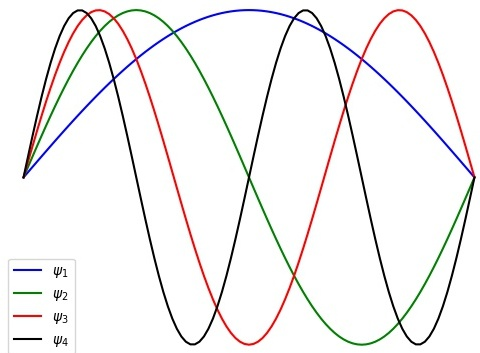
\includegraphics[width=0.6\textwidth]{aqm-6-sine}
	\end{center}
\end{figure}

Now imagine that we have many particles (bosons), some in state 1 (first energy level), some in second,..., which we will write: $\ket{n1,n2,n3,...}$. This is identical to the way we labelled states in a multi-oscillator system (We couldn't do this for Fermions!).  Because this is a complete parallel, we can \emph{invent} operators as in (\ref{eq:a:comm_i_plus}) - (\ref{eq:a:comm_i}) to \emph{literally} create and remove particles. NB $\set{1,2,3,...}$ are states, $\set{n_i}$ occupation numbers.

\begin{align*}
	a_1^+\ket{n_1,n_2,...} =& \sqrt{n_1+1} \ket{n_1+1,n_2,...}
\end{align*}
We had a question about the physical significance of the square root. We know that
\begin{align*}
	a^+a^-\ket{n} = n \ket{n} \numberthis \label{eq:creator:annihil}
\end{align*}
so it is reasonable to expect a square root to be associated with each operator. However, we can do better. Suppose that we don't know (\ref{eq:creator:annihil}), but we did know about commutator and square root.

\begin{align*}
	(a^+a^-)\ket{n}=&(a^-a^+-1)\ket{n}\\
	=&\sqrt{n+1}a^-\ket{n+1}-\ket{n}\\
	=&(\sqrt{n+1})^2\ket{n}-\ket{n}\\
	=&(n+1)\ket{n}-\ket{n}\\
	=&n\ket{n} \text{, which is  (\ref{eq:creator:annihil})}
\end{align*}

NB: we are \emph{defining} creation and annihilation operators. Don't ask \emph{why} for a definition, \emph{ask why it is useful}. E.g. our definition of creation is useful because we want to explore systems where the number of particles may change. It lets us create a photon, and annihilation lets us absorb particles.

\begin{defn}[Vacuum]
	Vacuum is the state that is annihilated by all annihilation operators: $a^-$ -- $\ket{0,0,0,....}$.
\end{defn}

Denote energy by $\omega_i$ for state $i$. 

\begin{align*}
	E =& \sum_{i} n_i \omega_i\\
	=& \sum_{i} \omega_i \underbrace{ a^+_i a^-_i}_\text{$N_i$} 
\end{align*}
You can think of this two ways:
\begin{itemize}
	\item oscillator energies;
	\item sum of all particles.
\end{itemize}

We are inventing something that is a bunch of oscillators.
\begin{itemize}
	\item a violin string is a bunch of oscillators;
	\item radiation in a cavity is a bunch of oscillators.
\end{itemize}
We are building up an idea of collections of particles as harmonic oscillators; soon enough we'll see the connection with fields.

We'll consider free particles--no interactions.

Why can we ignore ground-state energy? Because constants commute with everything. 

Quantum field theory is a book-keeping device for keeping track of many particles that come and go.

\subsubsection{Digression on History of  Quantum Field Theory }
\begin{itemize}
	\item Faraday invented Field Theory.
	\item Maxwell invented modern Field Equations (there had been wave eqiations before him).
	\item Planck introduced $\hslash$ (realized classical field theory not enough). He quantized the oscillators in cavity of black body: he didn't realize that field had to be quantized.
	\item Einstein realized field had to be quantized.
	\item Heisenberg, Pauli, Dirac put it all together around 1928.
	\item particle creation via harmonic oscillator? Maybe Dirac.
\end{itemize}

Quanta are the things that occupy the Occupation Numbers: if the field is the electromagnetic field we call the quanta photons.

\subsubsection{Quantum Field Theory resumed}
$\Psi(x)$ -- an operator that is a function of position--one operator for each position. It acts on a space of states $\{\ket{n_1,n_2,...n_i,...}\}$, known as \emph{Fock Space}--\cite{wiki:fock}.

\begin{align*}
	\Psi(x)\triangleq&\sum_{i}a^-_i\psi_i(x)\text{, not Hermitean, so conjugate is}\\
	\Psi^\dagger(x)=&\sum_{i}a^+_i\psi_i^*(x)\\
	\Psi(x)+\Psi^\dagger \text{ is}&\text{ Hermitean}
\end{align*}

If the $\psi$ were in the momentum representation, the coefficients would resemble Fourier coefficients. They are the quantum version of Fourier coefficients. 

What if we apply $\Psi^\dagger$ to vacuum? $\Psi(x)$ annihilates it--what about $\Psi(x)^\dagger$.

\begin{align*}
	\sum_{i} \ket{i} \bra{i} =& I \text{, sum over one particle states with $\psi_i$}\\
\sum_{i} \ket{i} \braket{i|X} =& \ket{X} \text{, state where particles known to be at $X$. But}\\
	\braket{i|X}=&\psi^*(X) \text{, so we can write:}\\
	\psi^*_i(x)\ket{i} =& \ket{x}\text{ one particle in state $i$ at $x$. But}\\
	\ket{i} =& a^+_i\ket{0} \text{, using $a^+_i$ to create the particle. Whence}\\
	\psi^*_i(x) a^+_i\ket{0}=&\ket{x}\\
	\Psi^\dagger(x) \ket{0} =& \ket{x}\text{ so $\Psi^\dagger(x)$ creates a particle at $x$.}
\end{align*}

\begin{itemize}
	\item $a^+_i$ creates a particle in state $i$.
	\item $\Psi^\dagger(x)$  creates a particle at position $x$.
	\item $a^-_i$ annihilates a particle in state $i$, or gives zero.
	\item $\Psi(x)$  annihilates a particle at position $x$, or gives zero.
\end{itemize}

There is a separate field for each Boson.

Add vacuum to a state, we get probability of 0.5 of vacuum, 0.5 of original state. It is not the same as zero. Vacuum has length of 1!

Let's make a two particle state, at $x$ and $y$. 
 
\begin{align*}
	\Psi^\dagger(y)\Psi^\dagger(y)\ket{0} =& \ket{y,x}\\
	\Psi^\dagger(x)\Psi^\dagger(y)\ket{0} =& \ket{x,y} \text{, but from (\ref {eq:a:comm_i_plus})}\\
	\Psi^\dagger(y)\Psi^\dagger(x) =& \Psi^\dagger(x)\Psi^\dagger(y) \text{, so}\\
	\ket{x,y} =& \ket{y,x} \text{, which is the defining property of Bosons.} 
\end{align*}

A given quantum field describes one type of Boson. There are two types of field for photons, as there are two polarizations. There is a separate field for each type of particle.

We can handle situation where number of particles is a random variable: a laser wave is a superposition of different number of photons.

\section{Quantum Field Theory II}

\subsection{Review construction of a simple quantum field}

The trick of introducing fields from particles can be done in two ways. We can start with particles and reconstruct why they can be described by fields, or start with wave fields and work out why they have quanta. Starting with particles we can describe 1 particle, 2 particles, etc, then move on to a variable number of particles. We'll start with one single type of particle. Number of photons in room changes constantly. A neuron can decay into a proton, an electron, and a neutrino. We can't rely on quantum mechanics of a single particle: we need to invent fields.

We will start with single particle quantum mechanics, a state vector $\ket{\psi}$. We can construct the inner product $\bra{x}\ket{\psi}=\psi(x)$ and the probability density $\psi^*(x) \psi(x)$.  Normalization: $\int \psi^*(x) \psi(x) dx=1$ gives \textit{number of particles}: this isn't very interesting since we had only one particle to begin with.

We next introduced some a particle states that form an orthonormal basis. There are many ways to do this. For instance the x-states form an orthonormal basis. The eigenvectors of any Hermitian operator will form a basis. In particular the energy eigenstates of the particles in a box--Figure \ref{fig:aqm-6-sine} form an orthonormal basis. 
\begin{align*}
		\int d(x) \psi^*_i(x) \psi_j(x) =& \delta_{i,j} \numberthis \label{eq:orthog:psi}
\end{align*}
Now we have another useful little manipulation. 

\begin{thm}[Construction of delta function from orthonormal basis]\label{thm:orthonormal}
	For any orthonormal basis, $\psi_i$, and any $x$ and $y$:
	\begin{align*}
		\delta(x-y)=& \sum_{i} \psi_i(y) \psi^*_i(x)
	\end{align*}
\end{thm}

\begin{proof}
	\begin{align*}
		\sum_{i} \ket{i} \bra{i} =& I \text{. For any $x$ and $y$}\\
		\braket{y|x}=& \sum_{i} \braket{y|i} \braket{i|x}\\
		=& \sum_{i} \psi_i(y) \psi^*_i(x) \text{, but}\\
		\braket{y|x}=&\delta(x-y) \text{, whence}\\
		\delta(x-y)=& \sum_{i} \psi_i(y) \psi^*_i(x)
	\end{align*}
\end{proof}

This is true for any set of eigenvectors of any Hermitian operator.

Now we move on to problem of studying many particles at the same time. How are we going to characterize a state? One set of states that is particularly useful is to say how many there are for each energy level. Characterize by the occupation numbers,  $\ket{n_1, n_2,...n_i,...}$. These don't belong in the same vector space s the single particle wave functions. Do not confuse the single particle states with these more general structures. We use the same notation merely because nobody has invented anything that works better than Dirac's bras and kets.

We want to change the numbers of particles, i.e. increase and decrease occupation numbers. We introduce an oscillator for each $i$: this has nothing to do with oscillation, it is just a bookkeeping trick. We introduce creation and annihilation operators, $a^+_i$ and $a^-_i$, and make them behave the same as the oscillator creation and annihilation operators. They are often written slightly differently.

\begin{itemize}
	\item $a^+_i=a^\dagger_i$
	\item $a^-_i=a_i$
\end{itemize} 

We will find it convenient to introduce the field operator, which operates on Fock space.
\begin{align*}
	\Psi(x) \triangleq & \sum_{i} a_i \psi_i(x)\\
	\Psi^\dagger(x) \triangleq& \sum_{i} a^\dagger_i \psi^*_i(x)
\end{align*}

\begin{itemize}
	\item These would be Fourier transforms if sine/cosine waves, except they are operator values, not numeric.
	\item $\Psi(x)$ and $\Psi^\dagger(x)$ are not Hermitian.
\end{itemize}

The following are Hermitian, and, hence, observable:
\begin{align*}
	\Psi(x) + \Psi^\dagger(x) \\
	\frac{\Psi(x) - \Psi^\dagger(x)}{i}
\end{align*}
But right now we aren't observing them, just using them as bookkeeping devices.

We will now look at a different interpretation of $\Psi(x)$. What does it do when it operates on the vacuum, the Fock space state where all the occupation numbers are zero: $\ket{0} = \ket{0,0,0,.....}$? We'll write down the following formula.

\begin{align*}
	\ket{x}=&\sum_{i}\ket{i}\braket{i|x}\text{ "resolution of the identity". Now}\\
	\ket{i}=&a^\dagger_i\ket{0} \text{, i.e. a state with one particle in $i^{th}$ energy level, and}\\
	\braket{i|x}=&\psi_i(x) \text{, so}\\
	\ket{x}=& \sum_i \psi^*_i(x)a^\dagger_i\ket{0}\\
	=& \Psi^\dagger(x) \ket{0}
\end{align*} 

So $\Psi^\dagger(x)$ is the operator that creates, out of the vacuum, a particle with position $x$.

\begin{itemize}
	\item $a^\dagger_i$ creates particles with definite energy;
	\item $\Psi^\dagger$ creates particles at definite locations.
\end{itemize}

Dirac introduced the following terminology:
\begin{itemize}
	\item c-number (an ordinary number) commutes with everything;
	\item q-number (quantum operator "number") does not always commute.
\end{itemize}

\subsection{Some illustrative calculations}
We will now see what we can do with the  $\Psi$ and  $\Psi^\dagger$ operators.

\subsubsection{Density of particles}

The operator $\int dx \Psi^\dagger(x) \Psi(x)$ is interesting: it is not the same as $\int dx \psi^\dagger(x) \psi(x)$ (operator vs wave function). What does it do?
\begin{align*}
	\int dx \Psi^\dagger(x) \Psi(x)=&\int dx \sum_{i,j}a^+_i\psi_i^*(x) a_j\psi_j(x) \text{, expanding using definition of $\Psi$ and $\Psi^\dagger$}\\
	=&\sum_{i,j} a^+_i a_j \int dx \psi_i^*(x) \psi_j(x)\\
	=&\sum_{i,j} a^+_i a_j \delta_{i,j} \text{, from (\ref{eq:orthog:psi})}\\
	=&\sum_i a^+_i a_i \text{. Now we use (\ref{eq:number:operator})}\\
	=&\sum_i N_i \text{, total number of particles.}
\end{align*}
So $\int dx \Psi^\dagger(x) \Psi(x)$ is the operator representing total number of particles. Will it be finite, since there are infinitely many $i$s? Unless the total energy is insanely high, the $N_i$ must fall off quickly. To make energy finite, total number of particles must be finite. $\Psi^\dagger(x) \Psi(x)$ represents particle density\footnote{The measured value is not necessarily the probability; usually will be within $\sqrt{n}$ of probability.}, since its integral is the total number.

Now  $\Psi^\dagger(x) \Psi(x)$ is an observable, so we can measure it.  To measure we integrate over a small volume, and ask how many particles are there. Like any observable it has states: you can measure and get a variety of answers.

$\{\ket{n_1,n_2,...n_i,...}\}$ is not the most general state: it is a basis. We can superpose to get the most general state.


\subsubsection{Total Energy}
We now determine the operator that gives the total energy. We'll assume that particles don't interact. This works for dilute particles. Even photons will interact if they are dense enough (we can't get this density in the laboratory.)

\begin{align*}
	E =& \sum_{i} N_i \omega_i \text{ sum over all modes, i.e. single particle states}\\
	=& \sum_{i} a^\dagger_i a_i \omega_i
\end{align*}

We determine $\omega_i$ from eigenvalues of the time independent Schr\"odinger equation (ignoring interactions). Particles may interact with $V$, but not with each other.
\begin{align*}
	H \psi_i =& \omega_i \psi_i\\
	\big[\frac{p^2}{2m} + V(x)\big]\psi_i(x)=& \omega_i \psi_i(x)\\
	\big[-\frac{\nabla^2}{2m} + V(x)\big]\psi_i(x)=& \omega_i \psi_i(x) \numberthis \label{eq:schroedinger:psi}
\end{align*}

We will guess the solution. Start with the observation that the expectation of the energy for one particle is given by:
\begin{align*}
	\braket{\psi | H | \psi} =& \big[-\frac{\nabla^2}{2m} + V(x)\big]\psi_i(x)
\end{align*}

This suggests:
\begin{thm}[Energy of multi-particle system]
	\begin{align*}
		E=&\int dx \Psi^\dagger(x) \big[-\frac{\nabla^2}{2m} + V(x)\big] \Psi(x)
	\end{align*}
\end{thm}

\begin{proof}
	\begin{align*}
		&\int dx \underbrace{\Psi^\dagger(x) \big[-\frac{\nabla^2}{2m} + V(x)\big] \Psi(x)}_\text{energy density} \\
		=& \int dx \sum_{i,j}a^+_i\psi_i^*(x)\big[-\frac{\nabla^2}{2m} + V(x)\big]\psi_j(x)a^-_j\\
		=& \int dx \sum_{i,j} a^+_i a^-_j \psi_i^*(x) \omega_j \psi_j(x) \text{, from (\ref{eq:schroedinger:psi})}\\
		=& \sum_{i,j} a^+_i a^-_j \delta_{i,j} \omega_j \text{, since $\{\psi_i\}$ form an orthonormal basis} \\
		=& \sum_{i} a^+_i a^-_i  \omega_i\\
		=& \sum_i N_i \omega_i
	\end{align*}
\end{proof}

Notes:
\begin{itemize}
	\item We can recover single particle QM from QFT: just go to states where total number of particles is one.
	\item Behaves like classical theory if the number of particles in same state is very large. E.g. expectations follow  laws of classical particles.
	\item If we don't split too many hairs,square of electromagnetic field is qualitatively related to density of photons.
\end{itemize}

You can imagine how confused everybody was before Dirac put it all together. People were confused by $psi$, which they thought was a field, like the electromagnetic field. Some thought it was just an auxiliary device for computing probabilities. If that was what is was, how was it connected with electromagnetic field? What was connection between particles and fields. The Scr\"odinger equation looked a but like Maxwell's equations. But Maxwell's equations were not anything to do with probability amplitudes: they concerned measurable value of the field. But there was a connection, as the photons were quanta of the field. QFT is the resolution of that confusion.  

For electromagnetic field:
\begin{align*}
	\vec{\Psi} =& \vec{E} + i \vec{B}\\
	\vec{\Psi^*} =& \vec{E} - i \vec{B}\\
	\vec{\Psi} \vec{\Psi^*} =&\text{ energy density of photons: $E^2+B^2$}
\end{align*}
Density of photons isn't a good concept, but energy density is.

\section {Second Quantization}

\subsection{Digression on neutrinos}

If neutrinos have mass, and they mix, do they have the same mass? No. So how to mix and conserve energy?

Mass is energy. The eigenstates of energy are linear superpositions of eigenstates of something else, \emph{the type of neutrino}. The eigenstates of energy don't mix with each other, but they are mixtures themselves.

\subsubsection{A simple example}

Here is simple example. Imagine a particle trapped in the potential of Figure \ref{fig:aqm-7-potential}, and let's suppose for the sake of argument that the middle barrier very high, so, to a good approximation, particle is trapped on one side or t'other (ignore tunnelling). So we can treat particle as being on the left, say. In Figure \ref{fig:particle_mixed_left} we treat the barrier as a brick wall and ask what is the ground state. We might say that Figure \ref{fig:particle_mixed_left} shows the ground state: it has no nodes, is as smooth as possible, and has an energy, $E$. But there must be a second ground state, from symmetry--Figure \ref{fig:double:well}, with the same energy. These are two states that have apparently the same energy--except they don't. The two wave functions in Figure  \ref{fig:double:well} are not exactly eigenstates of the energy.

\begin{figure}[H]
	\caption{Double well potential with very high barrier}
	\begin{subfigure}{0.3\textwidth}
		\caption{Double well potential}\label{fig:aqm-7-potential}
		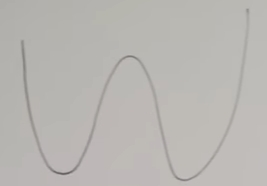
\includegraphics[width=0.8\textwidth]{aqm-7-potential}
	\end{subfigure}
	\begin{subfigure}{0.3\textwidth}
		\caption{One "ground state"}\label{fig:particle_mixed_left}
		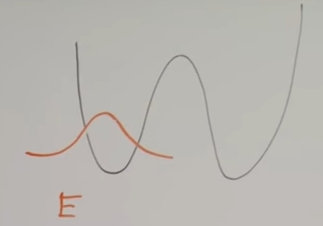
\includegraphics[width=0.8\textwidth]{particle_mixed_left}
	\end{subfigure}
	\begin{subfigure}{0.3\textwidth}
		\caption{Two "ground states"}\label{fig:double:well}
		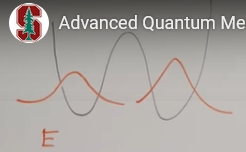
\includegraphics[width=0.8\textwidth]{particle_mixed}
	\end{subfigure}
\end{figure}

We know that for a potential like Figure \ref{fig:aqm-7-potential} the eigenstates are either symmetric or antisymmetric functions.

\begin{thm}[If $V$ is an even function, $\psi$ is either even or odd.]
	If  $\psi$  is a continuously differentiable solution to the time independent Schr\"odinger equation
	\begin{align*}
	-\frac{\hslash^2}{2m}\frac{d^2 \psi(x)}{d x^2} + V(x)\psi(x) =& E\psi(x) \text{ and}\numberthis \label{eq:ti:schroedinger}\\
	\forall x V(-x) =& V(x) \numberthis \label{eq:even_V}\\
	\text{then}&\text{ either}\\
	\psi(x) =& \psi(x)\text{, or}\\
	\psi(x) =& \psi(-x)
	\end{align*}
\end{thm}

\begin{proof}
	Define an operator $R$ (reflection in time) such that:
	\begin{align*}
		R \ket{\psi} =& \ket{\psi^{\prime}} \text{, where} \numberthis \label{eq:reflection}\\
		\psi^{\prime}(x) =& \psi(-x)
	\end{align*}
	
	(\ref{eq:even_V}) $\implies RV=V$, and $\psi^{\prime}$ satisfies (\ref{eq:ti:schroedinger}), whence:
	
	\begin{align*}
	\psi^{\prime}(x) =& \rho \psi(x) \text{, for some constant $\rho$.} \numberthis \label{eq:R:rho}
	\end{align*}
	WLOG we can assume that $\psi$ and $\psi^{\prime}$ are both normalized, whence:
	\begin{align*}
		\lvert \rho \rvert = 1& \text{, so (\ref{eq:reflection}) and (\ref{eq:R:rho}) give:}\\
		R \ket{\psi} =& \rho \ket{\psi} \text{. But (\ref{eq:reflection}) implies}\\
		R^2    =& I \text{, whence}\\
		\rho^2 =& 1 \text{, i.e.}\\
		\rho \pm& 1 \text{, so, in any interval where $\psi(x)\ne 0$ \emph{either}}\\
		\psi(x) =& \psi(-x) \text{\emph{or}}\\
		\psi(x) =& -\psi(-x)
	\end{align*}
	We still need to rule out the possibility that $\rho$ changes sign at a zero. Let $x_0$ be a point such that $\psi(x_0)=0$, and, WLOG, assume that $\psi(x)=\psi^{\prime}(x)$ in some interval up to $x_0-$ and $\psi(x)=-\psi^{\prime}(x)$ in some interval starting $x_0+$. Since $\psi$ is continuously differentiable: then $\frac{\psi^{\prime}(x_0-)}{dx}=\frac{\psi^(x_0-)}{dx}$. Now define $\psi^{\prime\prime} \triangleq \big(\psi^{\prime}-\psi\big)$: $\psi^{\prime\prime}$ satisfies (\ref{eq:ti:schroedinger}), $\psi^{\prime\prime}(x_0)=0$, and $\frac{\psi^{\prime\prime}(x_0-)}{dx}=0$, whence $\psi^{\prime\prime}=0 \forall x$. 
\end{proof}

But neither LHS or RHS wave function of Figure \ref{fig:double:well} symmetric or antisymmetric. Can make symmetric or antisymmetric combinations. Figure \ref{fig:double:well:symmetrized} has slightly lower energy than Figure \ref{fig:double:well}: it is the true ground state\footnote{Remember that sign of wave function doesn't matter}. Figure \ref{fig:double:well:1st} shows first excited state: it's energy is ever so slightly larger that a wave function constrained to be on one side.

\begin{figure}[H]
	\caption{Wave functions for Figure \ref{fig:double:well}}
	\begin{subfigure}{0.45\textwidth}
			\caption{Wave function symmetrized(minimum in middle is slightly greater than zero-allow tunnelling)}\label{fig:double:well:symmetrized}
			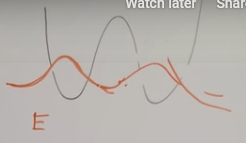
\includegraphics[width=0.8\textwidth]{particle_mixed_symmetrized}
	\end{subfigure}
	\begin{subfigure}{0.45\textwidth}
		\caption{First excited state}\label{fig:double:well:1st}
		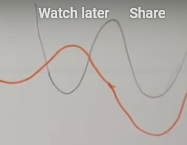
\includegraphics[width=0.8\textwidth]{particle_mixed_1st_excited}
	\end{subfigure}
\end{figure}


So we mix the pure states from Figures \ref{fig:double:well:symmetrized} and \ref{fig:double:well:1st}. Let's start with electron on left, and evolve.
\begin{align*}
	\frac{\psi_L+\psi_R}{\sqrt{2}}& \text{--symmetric, with energy }& E_1-\epsilon\\
	\frac{\psi_L-\psi_R}{\sqrt{2}}& \text{--antisymmetric, with energy }& E_1+\epsilon
\end{align*}
What if we put a particle on the left? How does it evolve? Each is an eigenvector, so they evolve as follows:
\begin{align*}
	\frac{\psi_L+\psi_R}{\sqrt{2}} e^{(E_1-\epsilon)t}=&\psi^+ \text{, say}\\
	\frac{\psi_L-\psi_R}{\sqrt{2}}e^{(E_1+\epsilon)t}=&\psi^-
\end{align*}

Now what if we start with pure $\psi_L$?
\begin{align*}
	\psi_L =& \frac{\psi^+ + \psi^-}{\sqrt{2}}\text{, then the denominator evolves as}\\
	\psi_L^\prime =&\psi^+ e^{(E_1-\epsilon)t} + \psi^- e^{(E_1+\epsilon)t}\\
	=&e^{E_1 t}\big[\psi^+ e^{-\epsilon t} + \psi^- e^{+\epsilon t}\big]
\end{align*}
Signs change with time, so eventually they will be opposite.
\begin{align*}
	e^{-\epsilon t} =& - e^{\epsilon t}\\
	e^{2 \epsilon t}=&-1\\
	2 \epsilon t = \pi
\end{align*}
So $\psi_L$ becomes $\psi_R$!

\subsubsection{Neutrinos}

The phenomenon of mixing goes with the phenomenon of oscillation. Neutrinos behave  like that: 
\begin{itemize}
	\item the analog of the left wave function is the neutrino that is made when a particle decays to an electron plus a neutrino;
	\item the analog of the right wave function is the neutrino that is made when a particle decays to a muon plus a neutrino.
\end{itemize}
The real eigenstate of the energy is a linear combination of the muon and electron neutrino. When a neutrino is made, it is either in a state of an electron neutrino or a muon neutrino. If you wait a while it will change to the other state.
--electron neutrino changes to muon neutrino.
Now the neutrino can be scattered, and produce an electron (from electron neutrino) or a muon. But wait a while and see what is produced: electron neutrino becomes muon neutrino, and can produce muons. This type of neutrino will oscillate! If you have a very long baseline you'll see the oscillations

What controls size of $\epsilon$? All sorts of details, mass of particle, height of barrier, width of barrier. It is extremely sensitive. 

The neutrino masses are the energy levels. They start small, but mixing splits the energy a bit. There is no barrier; there is a coupling in the Hamiltonian which, for whatever reason takes an electron neutrino to a muon neutrino and vice versa. In Figure \ref{fig:double:well} the coupling is due to tunnelling.

Ammonia has a tetrahedral shape--Figure \ref{fig:aqm-8-nh3}. The Nitrogen likes to sit a certain distance of the base of the triangle (energy lowest). But there is another state which is symmetric, with Nitrogen below: $N$ tunnels through $H_3$ plane. 

\begin{figure}[H]
	\begin{center}
		\caption{Ammonia has a tetrahedral shape}\label{fig:aqm-8-nh3}
		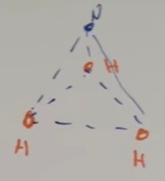
\includegraphics[width=0.5\textwidth]{aqm-8-nh3}
	\end{center}
\end{figure}

We've also seen this with spins. Without any magnetic field up and down have the same energy. Now apply a weak magnetic field--Figure \ref{fig:aqm-8-spins-lr}. What are the eigenstates? Left, and right. But these are just linear combinations of up and down.
\begin{align*}
	\ket{l} = \frac{1}{\sqrt{2}}\big[\ket{u} + \ket{v}\big]\\
	\ket{r} = \frac{1}{\sqrt{2}}\big[\ket{u} - \ket{v}\big]
\end{align*}
The eigenstates have slightly different energy because of the magnetic field: we have the same situation with slightly different energy levels. What happens if we start the electron up? It precesses, moving between down and up. There is no tunnelling, just a term in the Hamiltonian. 

\begin{figure}[H]
	\begin{center}
		\caption{Spins in a weak magnetic field}\label{fig:aqm-8-spins-lr}
		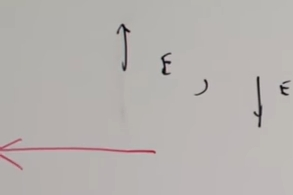
\includegraphics[width=0.5\textwidth]{aqm-8-spins-lr}
	\end{center}
\end{figure}

If there is something that an up electron can do, and down can't, and vice version, we can create the electron as an up, and later do an experiment to see whether it is behaving like a down.

The strength of field only controls speed of precession. The analogue of the magnetic field is the mixing of the neutrinos: this is a very small parameter, and we don't know where it came from. It doesn't fit into the Standard Model.

Neutrino oscillation: the energy is also affected by spin.

This is believed to be the explanation of the deficit of solar neutrinos: by the time they get here, some have transformed.

\subsubsection{Scientific American Article on whether electron is a sphere}

What would it mean for the electron to be a sphere?

What was measured was the electric dipole moment, the charge times the distance between them, and it represents an off centred distribution. The centre of the dumbbell is the centre. For a charge distribution not to have a dipole does not mean that it is a sphere. A charge distribution can have many multipole moments. What kind of shape corresponds to a dipole? One with an imbalance of charge. We could have a distribution shaped like an oblate spheroid, or any kind of ellipsoid. This would not have a dipole moment, because it is uniformly distributed about any plane passing through centre. It might have a quadrapole moment, or an octopole moment.

In quantum mechanics there is something odd about  the notion of spherical symmetry. Figure \ref{fig:aqm-8-qm-dumbbell} depicts a quantum dumbbell.
\begin{figure}[H]
	\caption{Quantum Dumbbells and electric dipoles}
	\begin{subfigure}[t]{0.3\textwidth}
		\caption{Quantum Dumbbell - e.g. a molecule}\label{fig:aqm-8-qm-dumbbell}
		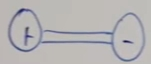
\includegraphics[width=\textwidth]{aqm-8-qm-dumbbell}
	\end{subfigure}
	\begin{subfigure}[t]{0.3\textwidth}
		\caption{Quantum Dumbbell - e.g. a molecule}\label{fig:aqm-8-qm-dumbbell-superposition}
		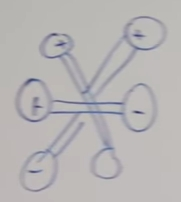
\includegraphics[width=\textwidth]{aqm-8-qm-dumbbell-superposition}
	\end{subfigure}
	\begin{subfigure}[t]{0.3\textwidth}
		\caption{Spinning electron, showing hypothetical imbalance of charge.}\label{fig:aqm-8-electron-spin}
		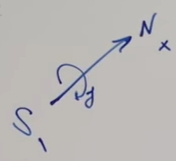
\includegraphics[width=\textwidth]{aqm-8-electron-spin}
	\end{subfigure}
\end{figure}
Let's take the ground state of the molecule, which is described by its angular momentum about the centre (ignore vibrations). If molecule is a boson, the ground state will have angular momentum $0$: wave function is completely symmetric for all rotations. So, independent of shape of molecule, the ground state is rotationally symmetric. Maybe it is a superposition of states, such as Figure \ref{fig:aqm-8-qm-dumbbell-superposition}, so wave function is symmetrized. Does Figure \ref{fig:aqm-8-qm-dumbbell-superposition} have a dipole moment? Answer is ambiguous, depending on the experiment.
\begin{itemize}
	\item Take a sudden quick snapshot; we'd discover it was lopsided with dipole moment. How fast does camera have to be? What resolution do we need? Snapshot measures angle; system would be in a state of definite orientation, so can't measure angular momentum (Heisenberg).
	\item What is energy of first excited state? What if it is enormous? More than we have in our photons. Then apparatus cannot resolve angle. We measure average: a sphere. Mesons are also (smaller) dumbbells. Kicking it into first excited state is huge compared to ordinary photons. All we can mesaud=sure shows it is a sphere on average.
\end{itemize}

Question of whether it a sphere or not is confusing.

Bosons can have spin zero, but electrons can't. They have an axis--Figure \ref{fig:aqm-8-electron-spin}. Given that direction, is there a charge imbalance?

What did they measure? Once you know that electron has an axis, we can ask whether there is an imbalance (small compared to overall negative charge--e.g. move charge from centre). Is there an imbalance as shown in Figure \ref{fig:aqm-8-electron-spin}? Is there a correlation between electrical charge displacement and the magnetic direction? This is what would be called the electric dipole moment of the electron.

Some symmetries forbid electric dipole moment, e.g. reflection symmetry. If the mirror image of an electron is another electron. Figure \ref{fig:aqm-8-mirror-image} shows that reflection doesn't preserve relationship between dipole and field direction. So, \emph{if the laws of physics don't distinguish between left hand and right hand}, there is no dipole moment.

\begin{figure}[H]
	\caption{Symmetries and dipoles}
	\begin{subfigure}[t]{0.45\textwidth}
		\caption[Mirror image of an electron]{Mirror image of an electron. Magnetic field has same directions, since it comes from spinning charge, but charge imbalance is reversed.}\label{fig:aqm-8-mirror-image}
		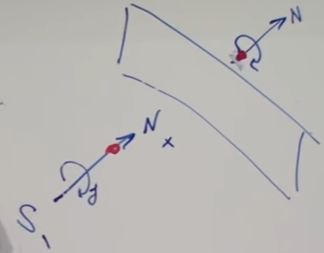
\includegraphics[width=0.8\textwidth]{aqm-8-mirror-image}
	\end{subfigure}
	\begin{subfigure}[t]{0.45\textwidth}
		\caption[Mirror image of an electron]{Mirror image of an electron. Magnetic field has same directions, since it comes from spinning charge, but charge imbalance is reversed.}\label{fig:aqm-8-time-reversal}
		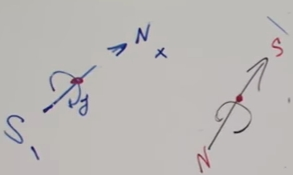
\includegraphics[width=0.8\textwidth]{aqm-8-time-reversal}
	\end{subfigure}
\end{figure}

But the laws of physics do distinguish between left hand and right hand (e.g. neutrinos). But there another more accurate symmetry, time reversal.  Figure \ref{aqm-8-time-reversal} shows the direction of spin being reversed, hence the magnetic filed reversed, but the charge distribution is unchanged. So time reversal would preclude a dipole, if it is a good symmetry of nature.

But time reversal is not a good symmetry of nature, either.

Standard Model predicts a very small dipole moment that is too small to detect. Experiment has failed to detect dipole moment.

\url{https://youtu.be/7G4C7scQX3A?t=4380}

\subsection{Second Quantization of Bosons}
 How are fields connected with Fourier transforms? In ordinary QM we have wave functions; in the position representation, and the squares define probabilities of the particle being at a particular point. We can Fourier transform the wave functions, and the transform is the representation in momentum space.


\begin{align*}
	\psi(x) \rightarrow& \psi^*(x)\psi(x)=&P(x) \text{ in position representation}\\
	\widetilde{\psi}(p) \rightarrow& \widetilde{\psi}^*(p) \widetilde{\psi}(p) =&P(p) \text{ in momentum representation, where}\\
	\widetilde{\psi}(p) =& \int \frac{dx}{\sqrt{2\pi}} \psi(x) e^{-i p x}\\
	\psi(x) =& \int \frac{dp}{\sqrt{2\pi}} \widetilde{\psi}(p) e^{+i p x}
\end{align*}

Now let's go to field theory, with creation and annihilation operators.

\begin{align*}
	\Psi(x) =& \sum_{i} a^-_i \psi_i(x)\\
	\psi_i(x) =& e^{ipx} \text{ for a free particle (different $i$!), so} \\
	\Psi(x)=& \int \frac{dp}{\underbrace{\sqrt{2\pi}}_\text{by convention}} a^-(p) e^{ipx} \text{, where annihilation operator}
\end{align*}
The momentum states are now represented by a continuous parameter, $p$, not a discrete $i$. Moreover $a^-(p)$  removes 1 particle with momentum $p$: it plays same role as $\widetilde{\psi}(p)$. If there is no particle to remove, $a^-(p)$ annihilates the state.
\begin{align*}
	\Psi^\dagger(x)=& \int \frac{dp}{\sqrt{2\pi}} a^+(p) e^{ipx} \text{ creates particle at position $x$}
\end{align*}
There is a similarity between wave functions in position and momentum space and creation and annihilation operators for particles and given position or momentum. And we can invert the equations.
\begin{align*}
	a^-(p) = \int \frac{dx}{\sqrt{2\pi}} \Psi(x) e^{-ipx}\\
	a^+(p) = \int \frac{dx}{\sqrt{2\pi}} \Psi^\dagger(x) e^{ipx}
\end{align*}

Remember there is a field operator for each kind of particle.

If we recall the commutators:
\begin{align*}
	[a^+_i,a^-_j] =& \delta_{i,j}\\
	[a^+_i,a^+_j] =& 0\\
	[a^-_i,a^-_j] =& 
\end{align*}
We can prove the following.
 
\begin{align*}
	[\Psi^+(x),\Psi^-(y)] =& \delta(x-y) \text{, introduces Heisenberg uncertainty!}\\
	[\Psi^+(x),\Psi^+(y)] =&0 \\
	[\Psi^-(x),\Psi^-(y)] =&0\\
	[\Psi^+_R(x),\Psi^-_I(y)] =& \delta(x-y) \text{, can not measure simultaneously at same point!}
\end{align*}

Makes sense in relativity: if measuring field at one point kicked value at a distant point, it would violate causality/locality. If there is a spacelike separation between measurements one cannot affect another!

Fermions don't work like this! One measurement can kick another arbitrarily far away. This sounds crazy--or there is no way to measure a Fermion Field.

\section{Quantum Field Hamiltonian}



\subsection{Particle Field Interactions}

In the previous lectures we talked about Quantum Fields, the quanta of those fields, the creation and annihilation operators, and examined the Hamiltonian for a very simple field--non-interacting particles satisfying Schr\"odinger's equation. The second term counts particles, giving each energy $V(x)$.\footnote{We are not restricted to 3D: x may be a vector.}
\begin{align*}
	H =& \int dx \big[ \Psi^\dagger(x) \big[\frac{- \nabla^2}{2m} \Psi(x) \big]+ V(x) \Psi^\dagger(x) \Psi(x) \big] 
\end{align*}
$\Psi^\dagger(x) \Psi(x)$ represents the density of particles at $x$, so $\Psi^\dagger(x) \Psi(x) V(x)$ counts particles at $x$, and gives each one energy $V(x)$.

We restrict to the special case of constant potential energy
\begin{align*}
H=&\int dx \big[\Psi^\dagger(x) \big(\frac{- \nabla^2}{2m} \Psi(x)\big) + mc^2 \Psi^\dagger(x) \Psi(x)\big]  \numberthis\label{eq:psi_mc2}
\end{align*}

Each particle has energy $mc^2$.

How do we see from (\ref{eq:psi_mc2}) that momentum is conserved?

The Hamiltonian updates state, $\phi$, say.

\begin{align*}
	\ket{\phi(t+\epsilon)} =& (1-i \epsilon H) \ket{\phi(t)} \text{State}\\
	=& \ket{\phi(t)} -i \epsilon H \ket{\phi(t)} \numberthis \label{eq:update:state}
\end{align*}

What would it mean to say momentum is conserved? It means Hamiltonian, when it acts on a state with definite momentum, doesn't change momentum. Whatever the Hamiltonian does, if it acts on a state with given momentum, it must give back the same momentum, \emph{if momentum is conserved.}  Let's see how this works with (\ref{eq:psi_mc2}). Rewrite 2nd term  using momentum variables (Fourier transform).

\begin{align*}
	\Psi(x) =& \int \frac{dp}{\sqrt{2\pi}} \underbrace{ \widetilde{\Psi}(p)}_\text{annihilation operator} e^{ipx}\\
	\Psi^\dagger (x) =& \int \frac{dp}{\sqrt{2\pi}} \underbrace{ \widetilde{\Psi}(p)}_\text{creation operator} e^{-ipx} \numberthis \label{eq:psi:dagger}
\end{align*}
 The factor is actually $\big(\frac{1}{\sqrt{2\pi}}\big)^n$ where $n$ is number of dimensions.
\begin{align*}
	\int dx \big(mc^2\big) \Psi^\dagger(x) \Psi(x) =& \frac{mc^2}{2 \pi} \int \widetilde{\Psi^\dagger}(p_2) \widetilde{\Psi}(p_1) e^{i(p_1-p_2)x} dx dp_2 dp_1\\
	=& \frac{mc^2}{2 \pi} \int \widetilde{\Psi^\dagger}(p_2) \widetilde{\Psi}(p_1) \delta(p_1-p_2) dp_2 dp_1\\
	=& \frac{mc^2}{2 \pi} \int \widetilde{\Psi^\dagger}(p) \widetilde{\Psi}(p) dp
\end{align*}

This just removes a particle with momentum $p$ and puts it back with same momentum; momentum isn't changed. The key thing was the integration over $x$, which introduced $\delta$ for momentum. Before we repeat with the 1st term of (\ref{eq:psi_mc2}) we will see that this can be more general. Let's suppose we had a term in the Hamiltonian for a whole bunch of fields: $\Psi^\dagger(x) \Psi(x)\rightarrow \Psi^\dagger_A(x) \Psi_A(x) + \Psi^\dagger_B(x) \Psi_B(x)+...$. We would end up with an integral:
\begin{align*}
	&\int dp_1A dp_1B...dp_2A dp 2B \Pi \Psi(p_1) \Pi \Psi(p_2) e^{i(\sum p_1-\sum p_2)x} dx\\
	=&\int dp_1A dp_1B...dp_2A dp 2B \Pi \Psi(p_1) \Pi \Psi(p_2) \delta(\sum p_1-\sum p_2) 
\end{align*}
The first sum is the momentum we put in, the 2nd the momentum that we take out. Total that we take out = total that we put in. Whenever we see a Hamiltonian of this form we have sum of outgoing momentum = sum incoming.

Let's look at derivatives. If we calculate $\nabla^2 \Psi^\dagger (x)$,  only one part of (\ref{eq:psi:dagger}) is affected, $e^{-ipx}$, since the remainder is doesn't involve $x$. 
\begin{align*}
	- \nabla^2 \Psi^\dagger (x) =& \int \frac{dp}{\sqrt{2\pi}} p^2 \widetilde{\Psi^\dagger}(p) e^{-ipx}\text{, so}\\
	\int dx \Psi^\dagger(x) \frac{- \nabla^2}{2m} \Psi(x)=& \int \frac{ p^2}{2m} \widetilde{\Psi^\dagger}(p) \widetilde{\Psi}(p) dp \numberthis \label{eq:minus:nabla}
\end{align*}
This adds the kinetic energy of all the particles.

Note: the left hand side of (\ref{eq:minus:nabla}) looks negative, but it is meant to be kinetic energy, which is positive. Integrating by parts we get:

\begin{align*}
	\int dx \Psi^\dagger(x) \frac{- \nabla^2}{2m} \Psi(x)=& \frac{1}{2m} \int dx \frac{\partial }{\partial x} \Psi^\dagger(x)  \frac{\partial }{\partial x} \Psi(x)
\end{align*}
This looks like any other Hamiltonian, where you see squares of derivatives of the fields. 

Imagine two species of particles: fake electrons and protons that happen to be bosons.\footnote{We aren't quite ready for Fermions.}

\begin{align*}
	H =& \int dx  \Psi^\dagger_e(x) \frac{- \nabla^2}{2m_e} \Psi_e(x) + \int dx \Psi^\dagger_p(x) \frac{- \nabla^2}{2m_p} \Psi_p(x)  + g \int dx \underbrace{\Psi^\dagger_e(x) \Psi^\dagger_p(x) \Psi_e(x) \Psi_p(x)}_\text{Figure \ref{fig:scatter:e:p}} 
\end{align*}
where $g$ is a coupling constant--proportional to probability of interaction. 

The integrand in last term annihilates a proton and an electron if it finds them at point $x$, then creates an electron and a proton.

\begin{figure}[H]
	\begin{center}
		\caption[$\Psi^\dagger_e(x) \Psi^\dagger_e(x) \Psi_e(x) \Psi_p(x)$--scattering]{$\Psi^\dagger_e(x) \Psi^\dagger_e(x) \Psi_e(x) \Psi_p(x)$: annihilate and create an electron and proton if they are at the same place, then create again --i.e. scatter}\label{fig:scatter:e:p}
		\feynmandiagram[vertical=o1 to i1]{
			i1[particle=$e^-$]--[fermion]a--[fermion]o1[particle=$e^-$],
			i2[particle=$p^+$]--[fermion]a--[fermion]o2[particle=$p^+$]
		};
	\end{center}
\end{figure}

\begin{itemize}
	\item Total momentum is conserved, not that of individual particles.
	\item Coulomb potential has been ignored.
	\item If experiment shows that particles interact, then there must be a term in the Hamiltonian.
	\item This is the sort of term for a short range interaction.
\end{itemize}

Imagine we find particle decay in an experiment, as shown in Figure \ref{fig:particle:decay}. We might try a term: $\Psi^\dagger_b(x) \Psi^\dagger_c(x) \Psi_a(x)$. Since space it isotropic, the interaction can happen anywhere: $g \int \Psi^\dagger_b(x) \Psi^\dagger_c(x) \Psi_a(x) dx$. We can show that momentum is conserved.

\begin{figure}[H]
	\caption{$\Psi^\dagger_b(x) \Psi^\dagger_c(x) \Psi_a(x) dx +  \Psi^\dagger_a(x) \Psi_c(x) \Psi_b(x)$}\label{fig:particle:decay:and:reverse}
	\begin{subfigure}{0.45\textwidth}
		\caption{Particle Decay: $\Psi^\dagger_b(x) \Psi^\dagger_c(x) \Psi_a(x)$}\label{fig:particle:decay}
		\feynmandiagram[horizontal' = b to c]{
			a[particle=a]--[charged scalar]cc--[charged scalar]b[particle=b],
			cc--[charged scalar]c[particle=c]
		};
	\end{subfigure}
	\begin{subfigure}{0.45\textwidth}
		\caption{Reverse: $\Psi^\dagger_a(x) \Psi_c(x) \Psi_b(x)$}\label{fig:particle:decay:reverse}
		\feynmandiagram[horizontal' = b to c]{
			b[particle=b]--[charged scalar]cc--[charged scalar]a[particle=a],
			c[particle=c]--[charged scalar]cc
		};
	\end{subfigure}
\end{figure}

Now what goes in the Hamiltonian must be Hermitian, so we need:
\begin{align*}
	g \int \Psi^\dagger_b(x) \Psi^\dagger_c(x) \Psi_a(x) dx + g \int \Psi^\dagger_a(x) \Psi_c(x) \Psi_b(x)
\end{align*}
which reverses the process of  Figure \ref{fig:particle:decay}: $b+c\rightarrow a$--Figure \ref{fig:particle:decay:reverse}.

We now have a the basic rules of a simple version of quantum field theory:
\begin{itemize}
	\item Creation and annihilation operators;
	\item Fields made out of creation and annihilation operators;
	\item Fields are functions of position;
	\item The Fields can be thought of as creation and annihilation operators at a definite position;
	\item Each type of particle has its own field;
	\item We write down Hamiltonian with kinetic energies of particles and other concoctions. 
\end{itemize}

In the first round of QFT the concoctions largely came from experiment. A classic example it beta decay: a neutron decaying into a proton, an electron, and a neutrino--$g \int \Psi^\dagger_{\nu}(x) \Psi^\dagger_e(x) \Psi^\dagger_p(x) \Psi_n(x) dx$ (need to make Hermitian).

Let's go one step further. Imagine that we made $\epsilon$ a little larger in (\ref{eq:update:state}):

\begin{align*}
	\ket{\phi(t+\epsilon)} =& \ket{\phi(t)} -i \epsilon H \ket{\phi(t)} - \frac{\epsilon^2}{2} H^2 \ket{\phi(t)}
\end{align*}

What is the effect of $H^2$? We can multiply it out, but the easy way is to use the pictures. E.g., Figure \ref{fig:particle:decay} becomes a scatter: $b+c \rightarrow a \rightarrow b + c$. Or Figure \ref{fig:scatter:annihilate} shows a more complex situation. You can have a forest of interactions that are mediated by a single term in the Hamiltonian. 

\begin{figure}[H]
	\caption{$\Psi^\dagger_c\Psi^\dagger_b\Psi_a\Psi^\dagger_a\Psi_b\Psi_c$}
	\begin{subfigure}[t]{0.45\textwidth}
		\caption{b and c scattering}\label{fig:scatter:annihilate}
		\feynmandiagram[horizontal' = b to c]{
			b[particle=b]--[charged scalar]cc--[charged scalar]a[particle=a],
			c[particle=c]--[charged scalar]cc,
			a--[charged scalar]ccc--[charged scalar]bb[particle=b],
			ccc--[charged scalar]cccc[particle=c]
		};
	\end{subfigure}
	\begin{subfigure}[t]{0.45\textwidth}
		\caption{Additional particle}\label{fig:additional:particle}
		\feynmandiagram[vertical = cc to c]{
			a[particle=a]--[charged scalar]cc--[charged scalar]b[particle=b],
			cc--[charged scalar]c[particle=c],
			bb[particle=b]--[charged scalar]c,
			c--[charged scalar]aa[particle=a]
		};
	\end{subfigure}
\end{figure}
\url{https://youtu.be/7a1hon7NJ1M?t=2917}


Figures \ref{fig:scatter:annihilate} and \ref{fig:additional:particle} have a coupling constant $g^2$.

What about $a\rightarrow (b+c)\rightarrow a$? This is a self energy diagram for $a$. A real $a$ has a probability of being a $b+c$, and it behave like a $b+c$ close together some times. Figure \ref{fig:self:energy:electron} shows a self energy diagram for the electron.

\begin{figure}[H]
	\caption[Scatter electron and emit photon]{Scatter electron and emit photon(field $A$):$A\Psi^+_e\Psi^-_e$. Sometimes what you thought was an electron behaves like an electron + photon. Don't take it too literally: this happens, then  this, then that. The pictures just come out of iterating the Hamiltonian twice. Low probability: think of as correction to structure of an electron, not a new process. If we look, we will screw up electron! Sometime you will see that what you thought was an electron is an electron + photon. Superposition.}\label{fig:self:energy:electron}
	\begin{subfigure}[t]{0.45\textwidth}
		\begin{center}
			\caption{Electron comes in and emits photon--$A\Psi^+_e\Psi^-_e$}
			\feynmandiagram[vertical=e2 to e1]{
				e1[particle=$e^-$]--[fermion]e2[particle=$e^-$]
				--[fermion]e3[particle=$e^-$],
				e2--[photon]x
	};
	\end{center}
	\end{subfigure}
	\begin{subfigure}[t]{0.45\textwidth}
		\begin{center}
			\caption{One other thing that can happen: emit photon and reabsorb. The photon is the electric field of the electron. If electron is moving at the speed of light it behaves like a suerposition of an electron and an electron+photon.}
			\feynmandiagram[vertical=e4 to e1]{
				e1[particle=$e^-$]--[fermion]e2--[fermion]e3
				--[fermion]e4[particle=$e^-$],
				e2--[photon,looseness=3.0,half left]e3
			};
		\end{center}
	\end{subfigure}
\end{figure}

Energy isn't just the sum of the particles: it includes these interactions.

We have just seen the basic physics: the rest is technology and tricks.



\subsection{The Dirac Equation}

We will study the relativistic electron. We will start with an electron that moves in 1 direction along a line. Why did Dirac want to handle the relativistic case? Electrons in at atom move at a significant proportion of the speed of light. 

\begin{align*}
	E =& \frac{p^2}{2m} \text {, classical}\\
	P =& -i \frac{\partial}{\partial x} \text{, quantum}\\
	H = & i \frac{\partial}{\partial t}\\
	E^2 =& p^2 + m^2 \text{, relativistic($c^2=1$). It becomes:}\\
	-\frac{\partial^2}{\partial t^2} \phi(x) =& -\frac{\partial^2}{\partial x^2}\phi(x) + m^2 \phi(x) 
\end{align*}

This was already known; it is the Klein-Gordon equation. But Dirac wanted this:
\begin{align*}
	i \frac{\partial \psi}{\partial t} =& H\psi\\
	=& \big(\sqrt{- \frac{\partial^2}{\partial x^2} + m^2}\big) \psi  
\end{align*}
What could this possibly mean? What is the operator on the right hand side? Dirac decided to start again. Imagine a particle moving along the x axis with the speed of light (massless).

\begin{align*}
	c P =& E \text{, moving to right. ($c=1$)}\\
	i \frac{\partial \psi}{\partial t} =& -i \frac{\partial \psi}{\partial x} \numberthis\label{eq:dirac1:R}\\
	\implies&\\
	\frac{\partial \psi}{\partial t} + \frac{\partial \psi}{\partial x}=&0
\end{align*}

Any function of x-t will satisfy this  equation. It describes a wave, moving to the right.

Three things are wrong with this equation:
\begin{enumerate}
	\item it allows particles with negative momentum, which have negative energy;\label{item:negative:energy}
	\item it only has particles that move to the right;\label{item:right:only}
	\item the electron has no mass, so it moves with the speed of light.\label{item:speed:light}
\end{enumerate}

Dirac solved second problem by imagining two species of electrons, one moving to the right, t'other to the left, labelled $\psi_1$ and $\psi_2$. Or a particle can be one or t'other, or a superposition.

\begin{align*}
	\frac{\partial \psi_1}{\partial t} + \frac{\partial \psi_1}{\partial x}=&0 \text{, moving to right}\\
	\frac{\partial \psi_2}{\partial t} - \frac{\partial \psi_2}{\partial x}=&0 \text{, moving to left}
\end{align*}

Imagine particle with two degrees of freedom, $x$ and $1/2$. Make second degree into matrix index. Introduce an observable, $\alpha$, to tell us whether particle is 1 or 2 (a bit like a spin). We thinks of the $\psi$s as a column vector, and introduce a matrix whose eigenvectors are $\psi_1$ or $\psi_2$. Here is such a matrix (observable).

\begin{align*}
	\underbrace{
		\begin{pmatrix}
			1 & 0\\
			0 & -1
		\end{pmatrix}
	}_\text{Dirac's $\alpha$}
	\begin{pmatrix}
		\psi_1\\
		\psi_2
	\end{pmatrix}\\
	H =& \alpha P \numberthis \label{eq:dirac:1d:hp}\\
	i\frac{\partial \psi}{\partial t} =& -i \alpha \frac{\partial \psi}{\partial x} \text{, matrix equation!}
\end{align*}

We have fixed problem \ref{item:right:only}, particles moving to the right only. To fix problem \ref{item:speed:light}, absence of mass, Dirac added a term to give the electron mass. 

\begin{align*}
	H =& \alpha P + \beta m \text{, where $\beta$ is some matrix. Now} \numberthis \label{eq:dirac:1D:m}\\
	E^2 =& P^2 + m^2 \text{, so}\\
	E^2 =& \big(\alpha P + \beta m \big) \big(\alpha P + \beta m \big)\\
	=& \underbrace{\alpha^2 P^2}_\text{(=1)} + \underbrace{\beta^2 m^2}_\text{set  $=1$} + (\alpha \beta + \beta \alpha) P m\\
	=&  P^2 + m^2 + (\alpha \beta + \beta \alpha) P m \text{, so we want:}\\
	\alpha \beta + \beta \alpha=&0 
\end{align*}

Now $\alpha$ is a Pauli matrix, $\sigma_3$, so we can use any other Pauli matrix for $\beta$. We will use
$
	\begin{pmatrix}
		0&1\\
		1&0
	\end {pmatrix}
$.

We have the 1-dimensional version of Dirac's equation.
\begin{align*}
	i \frac{\partial \psi}{\partial t}=& a p \psi + \beta m \psi \text{, where $\psi$ is a two component spinor.}\\
	i \frac{\partial}{\partial t}\begin{pmatrix}
	\psi_1\\
	\psi_2
	\end{pmatrix}=&-i \begin{pmatrix}
	1&0\\
	0&-1
	\end{pmatrix} \frac{\partial}{\partial x}\begin{pmatrix}
	\psi_1\\
	\psi_2
	\end{pmatrix} + \begin{pmatrix}
	0&m\\
	m&0
	\end{pmatrix}\begin{pmatrix}
	\psi_1\\
	\psi_2
	\end{pmatrix}
\end{align*}

So
\begin{align*}
	i\frac{\partial \psi_1}{\partial t} + i\frac{\partial \psi_1}{\partial x}=&m \psi_2\\
	i\frac{\partial \psi_2}{\partial t} - i\frac{\partial \psi_2}{\partial x}=&m \psi_1
\end{align*}

So the mass term couples the two equations, and makes particle move slower then light. Dirac knew that mass is coupled to ability to move left or right.

\section{Fermions and the Dirac equation}\label{section:fermions:dirac}

\subsection{Second Quantization of Fermions}

If you have two bosons, can put them into same state, and creation and annihilation operators commute. There is nothing strange about commuting, but anticommuting is odd. Suppose we have two particles, and we want to say that when we interchange them the wave function or state vector changes sign.  whose wave function changes sign when we interchange. Let $\ket{x,y}$ represent particles at x and y (two 3 dimensional positions). $\Psi^\dagger(x)\Psi^\dagger(y)\ket{0}$ will create.

For bosons, operators commute and:
\begin{align*}
	\ket{x,y}=&\ket{y,x} \text{, because}\\
	\Psi^\dagger(x)\Psi^\dagger(y)=&\Psi^\dagger(y)\Psi^\dagger(x) \text{, because}\\
	[\Psi^\dagger(x),\Psi^\dagger(y)]=&0
\end{align*}

For Fermions:
\begin{align*}
	\ket{x,y}=&-\ket{y,x} \text{, so we need}\\
	\Psi^\dagger(x)\Psi^\dagger(y)=& -\Psi^\dagger(y)\Psi^\dagger(x) \text{, or}\\
	\Psi^\dagger(x)\Psi^\dagger(y)+\Psi^\dagger(y)\Psi^\dagger(x)=&0 \text{. This is usually written:}\\
	\{\Psi^\dagger(x), \Psi^\dagger(y)\}=&0 \text{, where}\\
	\{A,B\}\triangleq& AB + BA \text{, the anticommutator.}
\end{align*}

In general we can go from Bosons to Fermions by replacing the commutator with the anticommutator.

NB  $\Psi^\dagger(x)\Psi^\dagger(x)=\frac{1}{2}\{\Psi^\dagger(x)\Psi^\dagger(x)\}=0$,  so we can't have two identical particles at same position.

\begin{itemize}
	\item For Bosons there is a clear distinction between creation and annihilation operators, since $[a,a^\dagger]=1$ (\ref{eq:a:comm_i}), and $[a^\dagger,a]=-1$. We can't confuse them because the spectrum of energies from $0$ to $\infty$ can't be turned upside down. Creation operators never give 0!.
	\item For Fermions $\{a^\dagger,a\}= \{a,a^\dagger\}=+1$: from the algebra there is no difference between creation and annihilation operators. They do different things, so they are different, but we can't see this from the algebra alone.
\end{itemize}

Consider occupation numbers of Fermion with only one state: creation operator takes $0$ to $1$; if we create again the operator  annihilates, leaving $0$. Complete symmetry between empty and filled, creation and annihilation (mathematically!--it doesn't mean they are the same).
\begin{align*}
	a^2=&0\\
	(a^\dagger)^2=&0
\end{align*}


\subsection{The Dirac Equation in 3 dimensions}

\subsubsection{Review of 1D Dirac Electron}

Returning to the 1D Dirac equation for zero mass, (\ref{eq:dirac1:R}):
\begin{align*}
	i \frac{\partial \psi}{\partial t}=& -i \frac{\partial \psi}{\partial x} \\
	H \Psi =& i \Psi
\end{align*}
This was a failure as a theory of 1D electrons. We want a 2nd species that propagates to the left.
\begin{align*}
	i \frac{\partial \psi_1}{\partial t}=& -i \frac{\partial \psi_1}{\partial x} \\
	H \Psi_1 =& i \Psi_1\\
	i \frac{\partial \psi_2}{\partial t}=& i \frac{\partial \psi_2}{\partial x} \\
	H \Psi_2 =& -i \Psi_2
\end{align*}
We combined into a vector, adding handedness, $\begin{pmatrix} \psi_1\\ \psi_2 \end{pmatrix}$, and defined the matrix $\alpha = \begin{pmatrix}
1&0\\
0&-1
\end{pmatrix}$

So we had (\ref{eq:dirac:1d:hp})
\begin{align*}
	H \psi =& \alpha P \psi
\end{align*}

That didn't get us a mass, but it got stuff moving in both directions. We then invented another matrix $\beta=\begin{pmatrix}
0&1\\
1&0
\end{pmatrix}$ and in (\ref{eq:dirac:1D:m}) wrote $H = \alpha P + \beta m$. Note $\alpha^2=\beta^2=1$, and $\alpha\beta + \beta\alpha=1$, whence $H^2=P^2+m^2$. We combined left moving and right moving, then added coupling to give mass. It is in this sense that a mass term switches you from left moving to right moving.

\subsubsection{The Dirac Equation in 3 dimensions}

 How do we do this in 3D? Let's  drop $m$ temporarily, make $\alpha$ a vector, $\vec{\alpha}$, so we can dot product with $\vec{P}$.
\begin{align*}
	H =& \vec{\alpha} \boldsymbol{\cdot} \vec{P}\\
	=& \alpha_x P_x + \alpha_y P_y + \alpha_z P_z \text{. We want}\\
	H^2 =& P_x^2 + P_y^2 + P_z^2
\end{align*}
So we need
\begin{align*}
	\alpha_x^2 =&1\\
	\alpha_y^2 =&1\\
	\alpha_z^2 =&1
\end{align*}
and
\begin{align*}
	\alpha_y\alpha_x + \alpha_x\alpha_y=&0\\
	\alpha_z\alpha_x + \alpha_x\alpha_z=&0\\
	\alpha_x\alpha_y + \alpha_y\alpha_z=&0
\end{align*}
which can be written:
\begin{align*}
	\{\alpha_y,\alpha_x\} =&0\\
	\{\alpha_z,\alpha_x\} =&0\\
	\{\alpha_x,\alpha_y\} =&0
\end{align*}

Dirac needed three matrices that satisfy these equations; the three Pauli matrices do exactly that:
\begin{align*}
	\vec{\alpha}=&\vec{\sigma} \text{, so}\\
	H =& \vec{\sigma} \cdot \vec{P}
\end{align*}

Spin is always $\pm 1$, so it looks as if we have two cases, where spin is either in the same direction as momentum, or the opposite; again we have a massless particle with positive and negative energy, and whose spin is locked so its axis is along the momentum vector.

Dirac's logic, which was not necessarily unimpeachable, was that he wanted to write an equation for H in terms or P without having an insane square root. He wrote $	H = \vec{\alpha} \cdot \vec{P}$ because he wanted it to be linear in the momentum. He wondered what $\alpha$ was, because it couldn't just be a bunch of numbers. By requiring $H^2=P^2$ he found the Pauli matrices. He thought that he had discovered the origin of spin. He was not correct it that it is not the case that every particles has to have spin, but he was right for Fermions.

We still have $H^2=P^2$, and we don't have a mass. So we try $H= H = \vec{\alpha} \cdot \vec{P}+\beta m$ for some $\beta$ such that $\beta^2=1$.

\begin{align*}
	H^2 = P^2 +& m^2 \\
	+& P_x m (\sigma_x \beta + \beta \sigma_x) \\
	+& P_y m (\sigma_y \beta + \beta \sigma_y) \\
	+& P_z m (\sigma_z \beta + \beta \sigma_z)
\end{align*}

So $\beta$ anticommutes with all the Pauli matrices: unfortunately there is not matrix that anticommutes with all the Pauli matrices.

\begin{thm}[There is no $2 \times 2$ matrix that anticommutes with the Pauli matrices]
	We can find 3 $2 \times 2$ matrices that anticommute, but not 4.
\end{thm}
\begin{proof}
	TBP
\end{proof}
We have two choices: we can give up, or introduce another 2 valued degree of freedom, so we would use $4 \times 4$. It turns out that this will work: $4 \times 4$ \emph{has nothing to do with space being 4 dimensional; it is just a mathematical fact about anti-commuting matrices.} 

There are many different and equivalent representation of the Dirac matrices, which must satisfy:
\begin{align*}
	\alpha_x^2=&1  \\
	\alpha_y^2=&1  \\
	\alpha_z^2=&1  \\
	\beta^2=&1
\end{align*}
and
\begin{align*}
	[\alpha_y,\alpha_z] =&0 \\
	[\alpha_z,\alpha_x] =&0 \\
	[\alpha_x,\alpha_y ]=&0 \\
	[\alpha_x,\beta]=&0 \\
	[\alpha_y,\beta]=&0 \\
	[\alpha_z,\beta]=&0 
\end{align*}
Here is one solution, the Pauli representation of the Dirac matrices. This is not the representation that Dirac used.
\begin{align*}
	\vec{\alpha} =& \begin{pmatrix}
		\vec{\sigma}&0 \\
		0&-\vec{\sigma}
	\end{pmatrix} \\ 
	\alpha_x =& \begin{pmatrix}
		\sigma_x&0\\
		0&-\sigma_x
	\end{pmatrix}=&\begin{pmatrix}
		0&1&0&0\\
		1&0&0&0\\
		0&0&0&-1\\
		0&0&-1&0
	\end{pmatrix}\\
	\alpha_y =& \begin{pmatrix}
	\sigma_y&0\\
	0&-\sigma_y
	\end{pmatrix}=&\begin{pmatrix}
		0&i&0&0\\
		-i&0&0&0\\
		0&0&0&-i\\
		0&0&i&0
	\end{pmatrix}\\
	\alpha_z =& \begin{pmatrix}
	\sigma_z&0\\
	0&-\sigma_z
	\end{pmatrix}=&\begin{pmatrix}
		1&0&0&0\\
		0&-1&0&0\\
		0&0&-1&0\\
		0&0&0&1
	\end{pmatrix}\\
	\beta =& \begin{pmatrix}
		0&1\\
		1&0
	\end{pmatrix} =& \begin{pmatrix}
		0&0&1&0\\
		0&0&0&1\\
		1&0&0&0\\
		0&1&0&0
	\end{pmatrix}
\end{align*}

When we tried $H= H = \vec{\alpha} \cdot \vec{P}+\beta m$, we found that for positive energy, $\sigma$ has to be aligned with momentum. We introduced another species which has its spin reversed: this is said to be the opposite \emph{chirality}.

\begin{defn}[Helicity]
	 Physically, the helicity operator can be thought of as a projection operator of spin along the direction of motion $h=\frac{\vec{S}\cdot\vec{P}}{\lvert P \rvert}$.
\end{defn}
\begin{defn}[Chirality]
	Chirality is the relationship between the directions of spin and momentum. If the directions are the same, the chirality is right handed, otherwise left handed.\cite{meredith2018helicity}
\end{defn}

We coupled the left and right handed particles using the off diagonal entries in $\beta$, and the mass. So mass is a coupling between left and right. For massless particles, chirality is conserved.[Sort out helicity]

What is $\alpha$? Each component of $\alpha$ is a matrix, with two eigenvalues $+1$ and two $-1$. What physical quantity does it represent? They don't commute, so we can't measure them simultaneously. What is physical meaning of a component? It is the velocity, so the expectation value in any state is the velocity of the particle.

For any operator $L$:
\begin{align*}
	\dot L =& i [H,L] \text{, for any operator L. We'll consider}\\
	\dot X =& i[\alpha P + \beta m,X]\\
	=& i \alpha [P,X]\\
	=&\alpha_x
\end{align*}

So it is the velocity of particle! Velocity is not the same as momentum for electron.

\begin{align*}
	\frac{d}{dt} \alpha_x=&[H,\alpha_x]\\
	 \ne& 0 \text{ because H contains $\alpha_y$ and $\alpha_z$}
\end{align*}
so $\alpha_x$ is not conserved.

It does a spiral movement called Zitterbewegung.

Dirac discovered a multiplicity of different states of the electron, one had to do with chirality, the other to do with actual spin.

\subsubsection{Dirac Electron  and negative energy}
Dirac equation can have negative energy, even in 1 D case. We don't need 3D even for interesting effects.

\begin{align*}
	H=P \text{, right moving electron, What if $P<0$?}
\end{align*} 

Ground state has lowest energy (not fewest particles). With negative energy can lower indefinitely! What does -ve energy mean? They are very dangerous, because ground state is lowest energy: if we have negative energies could lower energy past vacuum! Or we could lower energy indefinitely. 

Dirac \emph{defined} vacuum to have lowest energy. Dirac filled with negative energies (Fermions!) --only one in each state. Since they are Fermions, if state filled we can't keep going. Vacuum must have every negative state occupied; then thee is no room to lower energy further. Can add positive energy electron, or move a negative energy electron to positive--Figure \ref{fig:dirac:sea}. (This was an intuitive way to describe some mathematics).

In Figure \ref{fig:ds} we have filled all negative energy levels, whch stabilizes vacuum. We can put in a positive energy electron, Figure \ref{fig:aqm-10-dirac-sea}, or take out a negative energy electron and leave a hole, Figure \ref{fig:dirac:sea}
\begin{figure}[H]
	\begin{center}
		\caption{The Dirac Sea}\label{fig:ds}
		\begin{subfigure}[t]{0.3\textwidth}
			\begin{center}
				\caption{Positive energy electron added}\label{fig:aqm-10-dirac-sea}
				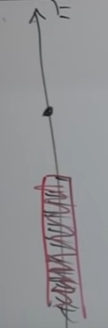
\includegraphics[width=0.5\textwidth]{aqm-10-dirac-sea}
			\end{center}
		\end{subfigure}
		\begin{subfigure}[t]{0.3\textwidth}
			\begin{center}
				\caption{Pluck out negative energy electron and get +ve charge and +ve energy hole (positron)}\label{fig:dirac:sea}
				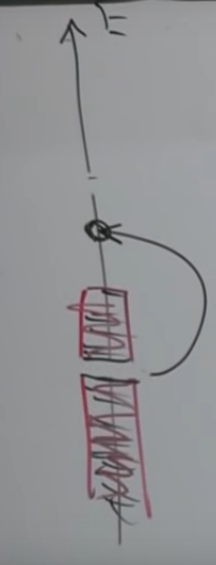
\includegraphics[width=0.5\textwidth]{DiracSea}
			\end{center}
		\end{subfigure}
		\begin{subfigure}[t]{0.3\textwidth}
			\begin{center}
				\caption{Photon displaces negative energy electron and produces +ve charge and +ve energy hole (positron)}\label{fig:dirac:sea:photon}
				\includegraphics[width=\textwidth]{aqm-10-dirac-sea-photon}
			\end{center}
	\end{subfigure}
	\end{center}
\end{figure}

Imagine photon coming along and hitting -ve energy electron in vacuum: we get an electron and a hole--Figures \ref{fig:dirac:sea:photon} and \ref{photon:dirac}.

\begin{figure}[H]
	\begin{center}
		\caption[Photon$\rightarrow$ electrons + hole]{Photon$\rightarrow$ electons + hole. By convention positron points down. Can slice in time: upwards electron, down positrons.}\label{photon:dirac}
		\feynmandiagram[vertical=n1 to i1]{
			i1--[photon,edge label=$\gamma$]n1--[anti fermion]o1[particle=$e^+$],
			n1--[fermion]o2[particle=$e^-$]
		};
	\end{center}
\end{figure}

The wave function needs fermion operators, which anticommute.
\begin{align*}
	\Psi =& \int_{-\infty}^{\infty} dp a^-(p) e^{-ipx}\\
	=& \underbrace{\int_{-\infty}^0 dp a^-(p) e^{-ipx}}_\text{negative energies}+ \underbrace{\int_0^{\infty} dp a^-(p) e^{-ipx}}_\text{positive energies}
\end{align*}

But the mathematics doesn't distinguish between Fermion creation and annihilation operators. Introducing $b^+(p)$, the creation operator for positirons:
\begin{align*}
	\Psi =&  \int_0^{\infty} dp  b^+(p) e^{ipx}+ \int_0^{\infty} dp a^-(p) e^{-ipx}
\end{align*}

Consider the interaction of Figure \ref{fig:electron_scattering_dirac}.
\begin{align*}
	a^+a^-A& \text{, which comes from a term in the Hamiltonian:}\\
	\Psi^\dagger(x)\Psi(x)A&\text{, }
\end{align*}

But this also describes the interactions of  Figures \ref{fig:electron_scattering_dirac}, \ref{fig:positron annihilating_dirac}, and \ref{fig:all3-created}.
\begin{figure}[H]
	\caption{Possible outcomes of $\Psi^\dagger(x)\Psi(x)A$: Feynman diagrams.}
	\begin{subfigure}{0.3\textwidth}
		\caption{Electron scattering}\label{fig:electron_scattering_dirac}
		\feynmandiagram[vertical'=a to i1]{
			i1[particle=$e^-$]--[fermion]a--[fermion]o1[particle=$e^-$],
			a--[photon]o2
		};
	\end{subfigure}
	\begin{subfigure}{0.3\textwidth}
		\caption{Positron annihilation}\label{fig:positron annihilating_dirac}
		\feynmandiagram[vertical'=i2 to a]{
			a -- [boson]b,
			c[particle=$e^-$]--[fermion]b,
			d[particle=$e^+$]--[anti fermion]b
		};
	\end{subfigure}
	\begin{subfigure}{0.3\textwidth}
		\caption{Electron, photon, positron created}\label{fig:all3-created}
		\feynmandiagram[vertical=o2 to i1]{
			a--[opacity=0.0]b,
			a--[fermion]c[particle=$e^-$],
			a--[anti fermion]d[particle=$e^+$],
			a--[boson]e,
			a--[opacity=0.0]f,
			a--[opacity=0.0]g
		};
	\end{subfigure}
\end{figure}

This was pretty much the start of Feynman diagrams (back in Dirac's day)! But Feynman figured out how to evaluate them.

How do modern physicists think of the Dirac Sea? They just forget the Dirac sea and replace creation operators for negative energy with annihilators for positive.

Same pattern in solid state physics. If you have crystal with lots of electrons, put all electrons into lowest available states--ground state. We have the Fermi sea. Can take an energy out of sea and kick into higher state, leaving a hole which behaves like a particle. But Dirac did this first!

Question about Cosmological constant. Can think of it as energy in Dirac Sea, or zero point oscillation of field. Photons aren't thought of as part of Dirac sea, but they contribute $\frac{1}{2}\hslash\omega$ for every oscillating mode. For photons background energy is positive, for Fermions it is negative. You could think of them cancelling, but Fermions have mass, photons don't, so they don't cancel. You are always left with some huge amount of energy left over. 

Keep in mind that the only time zero point energy comes into anything is when that energy is gravitating. For all other purposes we can ignore it because only differences matter.

% glossary: may need command make.glossaries.exe cosmology
\printglossaries

\bibliographystyle{unsrt}
\addcontentsline{toc}{section}{Bibliography}
\raggedright
\bibliography{tm}

\end{document}